% !TEX program = xelatex
% !TEX root = main.tex
\documentclass[black,normal,cn,hide]{elegantbook}

\usepackage{pdflscape}
\usepackage{tabu}
\usepackage{booktabs} 
\usepackage{colortbl} 
\usepackage{xcolor} 
\usepackage{xfrac}
\usepackage{tikz}
\usepackage{titling}
\usepackage{bytefield}
\usepackage{longtable}
\usepackage{graphicx}
\usepackage{float} 

\newcommand{\artdate}{2022年8月}
\newcommand{\artauthor}{陈泱宇,李燕琴}
\newcommand{\cpuname}{CDIM}
\newcommand{\cpuurl}{https://github.com/Maxpicca-Li/CDIM/blob/cyy_vipt_test/}
\newcommand{\arttitle}{CQU Dual Issue Machine 决赛设计报告}
\newcommand{\todo}{\textbf{\textcolor{red}{此部分尚需完善。}}}
\newcommand{\hlrule}{\rule{\linewidth}{0.5mm}}
\renewcommand{\maketitlehooka}{\null\mbox{}\vfill}
\renewcommand{\maketitlehookd}{\vfill\null}


\graphicspath{{img/}}
% 页眉设置
\pagestyle{fancy}
\fancyhf{}
\rhead{\thepage}
\lhead{\arttitle}
\cfoot{\thepage}

\begin{document}

\begin{titlepage}
    % \rule{\linewidth}{0.5mm}
    \vfill
    \center 
    \textit{\Large “龙芯杯”第六届全国大学生计算机系统能力培养大赛}\\[0.5cm] 
    \texttt{\Large 重庆大学 “所以延迟槽会消失对不队”队}
  
    \vspace{1.5 cm}
    \hlrule \\[0.4 cm]
    { \huge \bfseries \cpuname 项目}\\[0.4cm]
    { \huge \bfseries 决赛设计报告}\\
    \hlrule \\[1cm]
   
    \begin{figure}[h]
      \centering
      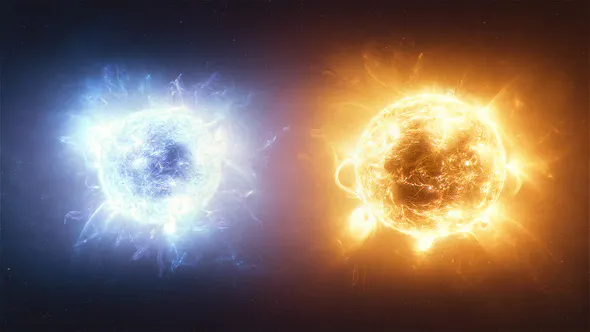
\includegraphics[width=0.5\linewidth]{logo.png}
    \end{figure}
   \vspace{0.5 cm}
  
    \vspace{.5 cm}
    陈泱宇\\
    cyy@cyyself.name\\
    \vspace{.5 cm}
    李燕琴\\
    maxpicca@qq.com\\
    \vspace{.5 cm}
    王梓宇\\
    925136384@qq.com\\
    \vspace{.5 cm}
    张翀\\
    20194159@cqu.edu.cn\\
  
    \vspace{2 cm}
    {\large \artdate}\\[3cm] 
  
  \vfill
  
\end{titlepage}

\tableofcontents
\mainmatter

% 可以使用input(但是无法显示outline),或直接在正文写
\chapter{概述}

\section{项目背景}
本项目依托于龙芯杯提供的FPGA实验平台、Soc工程环境以及基准测试程序,设计并实现了一个部分兼容 MIPS32 体系结构的小端序 CPU,名为CDIM(\textbf{C}QU \textbf{D}ual \textbf{I}ssue \textbf{M}achine),其能成功通过龙芯杯提供的功能测试、性能测试、系统测试,具有较完善的运算处理、AXI访问、异常处理、中断响应等功能,并能够运行u-boot引导程序、uCore操作系统和Linux操作系统等。

\section{名词解释}
本项目中可能用到的一些名词缩写及其解释如表\ref{table:abbreviation_definition}所示。

\begin{table}[!htbp]
    \centering
    \caption{名词缩写和解释}
    \label{table:abbreviation_definition}
    
    \begin{tabular}{cll}
    \toprule
    \multicolumn{1}{c}{\textbf{名词缩写}} & \multicolumn{1}{c}{\textbf{全称}}                   & \multicolumn{1}{c}{\textbf{解释}} \\ 
    \midrule
    MIPS                               & Microprocessor without Interlocked Pipeline Stages & 无内部互锁流水级的微处理器                \\
    SOC                                & System On a Chip                                   & 片上系统                             \\
    MIPS                               & Microprocessor without Interlocked Pipeline Stages & 无内部互锁流水级的微处理器 \\
    SOC                                & System On a Chip                                   & 片上系统 \\
    CPU                                & Central Processing Unit                            & 中央处理器 \\
    ALU                                & Arithmetic Logic Unit                              & 算数逻辑单元 \\
    GPR                                & General Purpose Register                           & 通用寄存器 \\
    CP0                                & Co-Processor 0                                     & 协处理器0 \\
    BRAM                               & Block Random Access Memory                         & 块随机访问存储器 \\
    FIFO                               & First In First Out                                 & 先进先出 \\
    RAW                                & Read After Write                                   & 写后读 \\
    WAW                                & Write After Write                                  & 写后写 \\
    WAR                                & Write After Read                                   & 读后写 \\
    \bottomrule
    \end{tabular}
\end{table}

\section{项目概述}
CDIM(\textbf{C}QU \textbf{D}ual \textbf{I}ssue \textbf{M}achine),采用对称双发射五级顺序流水线的设计,支持指令FIFO、分支预测、指令缓存和数据缓存等特殊单元,以提升系统性能。其中双发射,采用对称双发逻辑以充分保证双发率;五级顺序流水线由取指(Instruction Fetch)、译码(Instruction Decode)、执行(Excute)、访存(Memory access),写回(Write Back)五个阶段组成;指令FIFO可以隔离取指阶段和后续阶段,以实现高效取指的作用;指令缓存和数据缓存均采用二路组相联和突发传输的设计,单路均为4KB以匹配TLB页面要求,其中指令缓存一行为64bit以适应双发取指要求,数据缓存一行为32bit。\todo 此外,CDIM还支持U-Boot引导程序,并基于该引导程序,成功运行uCoreh和Linux操作系统。
% TODO: 系统运行这一段陈述
\chapter{CPU设计方案}

\cpuname 采用对称双发射顺序执行,共有5级流水。\cpuname 的数据通路示意图如\ref{img:datapath}所示,其中红线部分为Master Path,蓝线部分为Slave Path。在对称双发射中,Master和Slave的主要区别在于前者先于后者执行,在处理异常、提交等事宜时会被优先处理。当然,上述的“对称”双发射,只是相对于只支持ALU指令双发的非对称逻辑而言,\cpuname 的设计中Slave Path支持的功能和Master Path旗鼓相当。但严格来讲,并不是绝对对称,在处理跳转指令、例外指令、写TLB指令等这类可能刷新流水线的指令时,需要优先在Master处理,这在后续的双发策略中会详细说明。

% \begin{landscape} % 用于旋转页面
\begin{figure}[h]
    \centering
    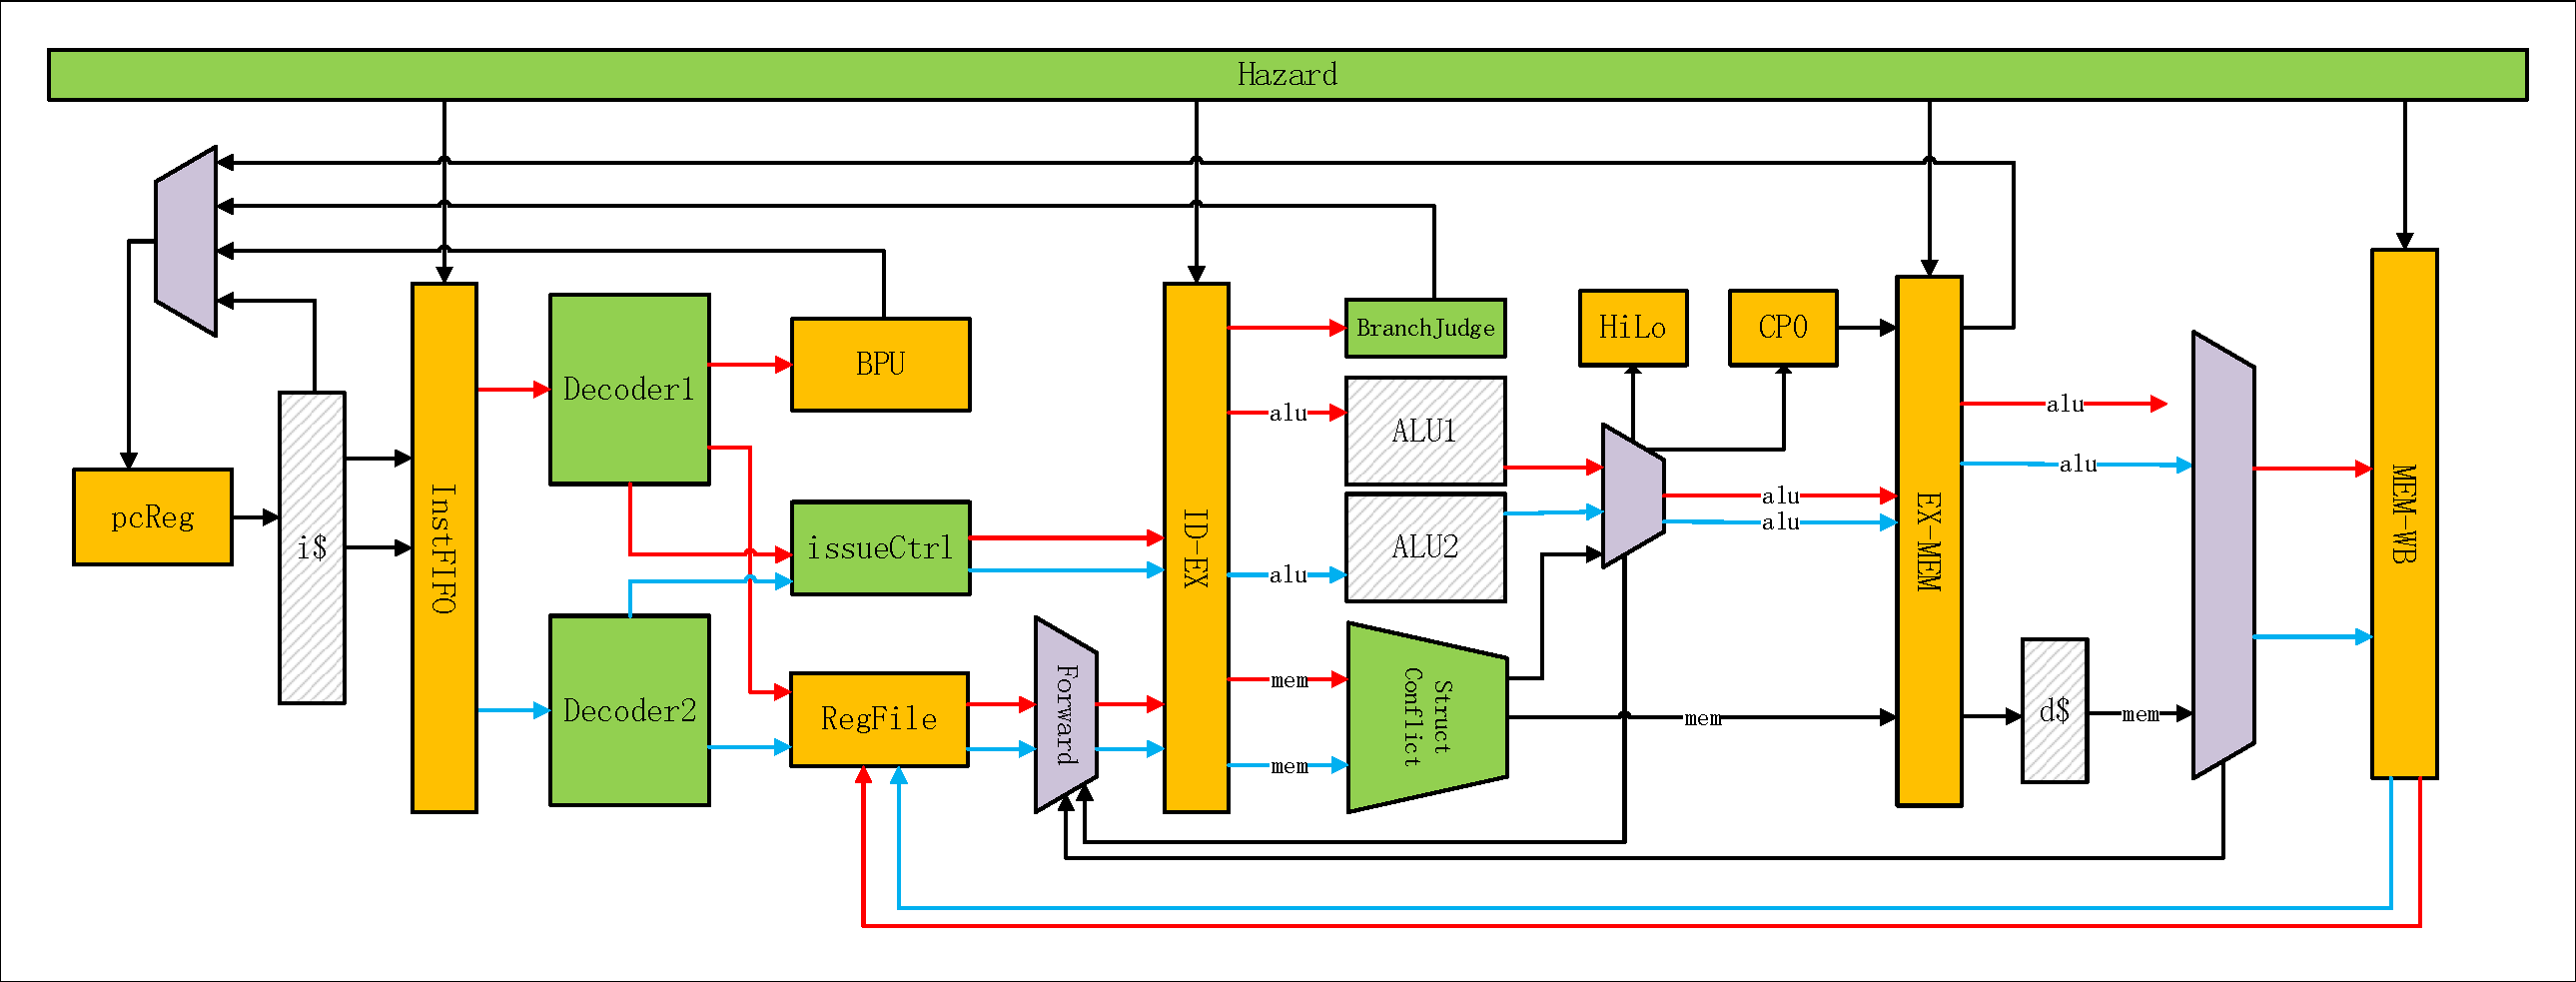
\includegraphics[width=\linewidth]{datapath.pdf}
    \caption{数据通路设计图}
    \label{img:datapath}
\end{figure}
% \end{landscape}


\section{指令集支持}
为了满足大赛提供的功能测试、性能测试、系统测试的要求以及运行操作系统需要的基本指令要求,我们实现了除Branch likely指令和浮点指令的所有 MIPS Release 1 指令集,按照功能分类如下。
\begin{itemize}
    \item \textbf{逻辑运算指令}:OR, AND, XOR, NOR, ORI, ANDI, XORI, LUI
    \item \textbf{移位指令}:SLL, SRL, SRA, SLLV, SRLV, SRAV
    \item \textbf{数据移动指令}:MFHI, MFLO, MTHI, MTLO, MOVN, MOVZ
    \item \textbf{算术运算指令}:ADD, ADDU, SUB, SUBU, SLT, SLTU, ADDI, ADDIU, SLTI, SLTIU, MULT, MULTU, MUL, MADD, MADDU, MSUB, MSUBU, DIV, DIVU, CLO, CLZ
    \item \textbf{跳转分支指令}:J, JAL, JR, JALR, BEQ, BNE, BGTZ, BLEZ, BGEZ, BGEZAL, BLTZ, BLTZAL
    \item \textbf{访存指令}:LB, LBU, LH, LHU, LW, SB, SH, SW, LWL, LWR, SWL, SWR, LL, SC
    \item \textbf{特权指令}:MFC0, MTC0, ERET, WAIT
    \item \textbf{自陷指令}:BREAK, SYSCALL, TEQ, TEQI, TNE, TNEI, TGE, TGEI, TGEU, TGEIU, TLT, TLTI, TLTIU, TLTU
    \item \textbf{Cache指令}:CACHE, PREF
    \item \textbf{TLB指令}:TLBP, TLBR, TLBWI, TLBWR
\end{itemize}

\section{双发策略}
在双发射的CPU设计中,双发策略会影响整个数据通路的设计,故我们先来介绍一下\cpuname 的双发策略,即分情况讨论Slave是否发射。在提供的代码中,issueCtrl模块解释了\cpuname 的整个双发策略。

\begin{enumerate}
    \item \textbf{only\_Master类指令}: 即只能放在Master发射,且Slave不发射指令。对于可能刷新整个流水线的指令(如MTC0、SYSCALL、ERET、BREAK、TLBWI、TLBWR等指令),如果在Slave中检测到这类指令,则暂停Slave发射,将其延迟到下一周期的Master发射;如果在Master中检测到这类指令,也会暂停Slave发射,避免不必要的流水线刷新。
    \item \textbf{only\_in\_Master类指令}: 即只能放在Master发射,且Slave可发射指令。 对于跳转指令,在一定条件下会跳转到其他地址,并刷新整个流水线。和only\_Master不同的是,跳转指令会涉及到延迟槽的处理。故如果在Slave中检测到这类指令,则暂停Slave发射,将其延迟到下一周期的Master发射;如果在Master中检测到这类指令,若满足Slave发射条件,则发射该条指令(延迟槽),若不满足,则在下一周期的Master中发射延迟槽数据。
    \item \textbf{数据冲突}
    \begin{enumerate}
        \item \textbf{RAW冲突}:检查Master和Slave之间是否存在HiLo、CP0、GPR等寄存器的RAW情况,若存在,则Slave不发射。
        \item \textbf{Load To Use 冲突}:检查Slave读到的寄存器是否是当前在E阶段执行的读存指令的结果,若是,则Slave不发射。
    \end{enumerate}
    \item \textbf{结构冲突}:由于设计的乘除单元、访存单元只有一个,故二者会产生结构冲突。若Master和Slave同时需要占用这类单元,则Slave不发射。
    \item \textbf{数据有效性}:Slave发射的前提是Master发射或当前第二条指令有效。若遇到Master暂停发射或指令FIFO为空的情况下,Slave不发射。
\end{enumerate}


\section{数据通路设计}
\subsection{取指阶段}
为了保证双发射能够正常执行,第一要素便是“一次取指能够取回多条指令”,才能保证传到D阶段时,至少有两条指令可以准备用于双发射。指令Cache数据行为64bit的设计,也正适应了双发逻辑中取指的特点,使得\cpuname 传入指令Cache一个PC地址,可获得该PC及PC+4对应的两条指令。值得注意的是,为了简化Cache命中逻辑(即不存在跨Cache Line访问Cache的情况),传回数据中,并不是所有PC都会传回2条指令,故我们添加了inst\_data\_ok信号表示取回的指令是否有效。\cpuname 的设计中,数据行共2字,如果PC索引到该行的最后一个字,Cache只传回1条指令,inst\_data\_ok2置为0;除此之外,传回两条数据,inst\_data\_ok1和inst\_data\_ok2均置为1。

出于双发策略中,Slave并不是每次都会发射,故取回的数据需要缓存下来,以用于下次使用,节省Cache访问时间。\cpuname 中,使用指令FIFO,将传回的有效指令缓存下来。使用指令FIFO还有一个好处是可以分割取指和后续阶段,即取指不受后续阶段产生的阻塞影响(但为了保证结果的正确执行并简化控制逻辑,后续阶段仍然会受到指令Cache产生的stall影响)。其中,如果指令FIFO放满,则暂停前段取指;如果指令FIFO为空,则暂停后续发射。

\subsection{译码阶段}
Instruction Decode阶段中,主要完成以下操作:
\begin{itemize}
    \item \textbf{译码}:从FIFO中读出指令,立即进入译码模块。译码模块中,会分析该指令的功能,并分配控制信号。
    \item \textbf{分支预测阶段}:为了减少分支跳转带来的流水线刷新数量,我们添加了静态分支预测单元,利用PC低位记录跳转数据,利用传统2bit策略更新跳转数据的记录。在D阶段获取到指令后,立即根据该指令所在PC进行预测,其中为了减少译码带来的延迟,分支预测单元内部单独进行分支译码,若是分支指令,即可取出预测结果并更新取指阶段的PC。
    \item \textbf{发射判断}:译码结束后,需要进入issueCtrl模块进行发射判断,发射判断结果会返回到指令FIFO中,控制FIFO的读指针的增量。
    \item \textbf{数据准备}:读取RegFile中对应的GPR数据,准备好数据后进入Excute阶段执行(在\cpuname 中,RegFile具有4个读端口和2个写端口)。其中为了在执行阶段的开头即可直接使用准确的数据,我们将数据前推单元放在了译码阶段的末尾。值得注意的是,为了减少前推带来的延迟,译码阶段中需要GPR数据的模块,均使用GPR直接读出的数据,而不是前推数据(如JR类指令目标地址的计算),若此时存在RAW冲突,则需要推迟到执行阶段进行计算。
\end{itemize}

\subsection{执行阶段}
Excute阶段中,主要完成以下操作:
\begin{itemize}
    \item \textbf{跳转处理}:在译码阶段中,Branch指令需要在执行阶段中判断跳转是否成功,并将判断结果送回分支预测单元进行数据更新,更新此时取值阶段的PC并刷新流水线。同理,如果是译码阶段遇到数据冲突的JR类指令,其在本阶段获取到准确的目标地址后,更新此时取值阶段的PC并刷新流水线。
    \item \textbf{ALU计算}:可以处理单周期运算指令和多周期运算指令。其中,多周期运算指令包括乘除法指令。\cpuname 中乘法指令需要2周期、除法指令需要35周期,且在运算完成前会产生stall信号(流水线阻塞信号),阻塞D、E、M、W四个阶段。其中,为减少资源占用,流水线中只提供一个乘法器和除法器,故Master和Slave在使用时需要进行仲裁。同时获取到乘除结果后,即在执行阶段写HiLo寄存器,以期在访存阶段即可获取新的HiLo数据值,避免了HiLo数据的前推。
    \item \textbf{访存仲裁及其地址计算}:由于Data Cache是BRAM结构,需要一个周期取出数据,我们需要在E阶段将访存信号传递给Data Cache。因为Master和Slave都支持访存(但不会同时访存),故在传递访存前,需要用StructConflict模块进行仲裁;并保证访存阶段的刷新信号置0且使能信号置为1,以使访存信号能由E阶段正常传到M阶段,保证访存阶段数据的正常传回。同时,为了减少访存地址计算经过的路径,我们分离了执行阶段中的ALU路径和MEM路径(如图 \ref{img:datapath} 所示),单独利用base(rs value) + offset(immediate value)计算访存地址。同时根据访存地址及其比特要求对传给Data Cache的地址进行地址错例外判断(AdEl和AdEs判断)。
    \item \textbf{TLB地址转换}:在上一个小点中,能够获取到访存虚拟地址,此时将访问 L1 TLB (TLB访问逻辑见章节\ref{section:TLB})进行初步的映射地址翻译,以便于提前访存。
    \item \textbf{异常汇总}:由上述可以看出,在执行阶段,可以获取从任何指令涉及到的所有异常信号,故我们在执行阶段汇总异常信号,并更新CP0寄存器,以期在访存阶段即可获取新的CP0数据值,避免了CP0数据的前推。
\end{itemize}

\subsection{访存阶段}
Memory Access阶段,主要完成以下操作:

\begin{itemize}
    \item \textbf{访存控制}:虽然在E阶段传递给了Data Cache基本的访存信号,告知Data Cache需要准备对应地址的数据;但是并没有告知需要取出的数据的比特数。E阶段汇总时若发现异常,则传到M阶段后,会将Data Cache的握手信号data\_sram\_enM(M阶段的访存使能信号)将会置为0,阻止Data Cache将错误的地址传到AXI总线上。反之,则正常发送data\_sram\_enM信号,并得到传回的数据,再通过StructConflict模块,将数据交付到对应 Path(Master或Slave)上。
    \item \textbf{写回数据选择}:Master和Slave两条路径上的计算结果(alu)和访存结果(mem)的选择。
\end{itemize}

\subsection{写回阶段}
Write Back阶段,主要执行写回GPR请求。若此时读取GPR的地址,恰好是写GPR的地址,需要进行写前递操作。

\section{冲突处理}
\subsection{数据冲突}
\begin{itemize}
    \item \textbf{RAW冲突}:当Master或Slave需要读取的数据是已经发射且进入后续流水阶段的指令,会产生RAW冲突。本设计将需要的数据均前推到D阶段,前推后立即进入触发器后再进入E阶段使用,这样可以避免执行数据的路径过长。其中,若需要读取的数据是当前E阶段的访存数据,则需要进行阻塞以等待访存数据在M阶段返回。若需要读取的数据是当前E阶段的计算结果、或M阶段的计算结果、或M阶段的访存结果,则通过数据前推模块前推到D阶段。
    \item \textbf{WAW冲突}:当同周期的Master和Slave写入寄存器的地址一致时,会产生WAW冲突。因为Slave是Master后一条指令,故RegFile更新时,会优先写入Slave的结果。
    \item \textbf{WAR冲突}:由于本设计为顺序流水线,故不存在WAR冲突。
\end{itemize}

\subsection{结构冲突}
当Master和Slave同时需要访存或占用乘法器或占用除法器时,会产生结构冲突。本设计中,结构冲突的指令只发射Master一条,保证CPU正确执行。

\subsection{控制冲突}
当遇到跳转指令时,会产生控制冲突。MIPS指令系统中,跳转指令包含延迟槽。本设计中,若产生跳转(译码阶段或执行阶段),则根据发射情况判断当前Path中的第一条读数据是否是延迟槽数据。如果是,则需要判断当时是否有阻塞信号,若没有则直接执行该第一条读数据,若有则需要保留该数据到指定delayslot\_data寄存器,以备阻塞取消后使用;此外跳转会引起流水线的刷新,但需要保证延迟槽数据能够不被刷新并正常流入下一阶段执行。如果不是,则正常刷新流水线即可。

\section{CP0寄存器}
在自定义CPU中扮演着小型操作系统角色的CP0,具有异常处理、内存管理、系统控制等功能。
为了支持MIPS指令系统的正常功能运行,我们设计的CP0处理器包含的基本寄存器如表\ref{table:base_cp0}所示。

\begin{table}[!htbp]
    \centering
    \caption{基本的CP0寄存器}
    \label{table:base_cp0}
    \begin{tabular}{ccll}
        \toprule
        \multicolumn{1}{c}{\textbf{编号}} & \multicolumn{1}{c}{\textbf{选择}} & \multicolumn{1}{c}{\textbf{名称}} & \multicolumn{1}{c}{\textbf{功能定义}} \\ 
    \midrule
    8   & 0 & BadVAddr  & 记录最新地址相关例外的出错地址 \\
    9   & 0 & Count     & 处理器内部计数器 \\
    11  & 0 & Compare   & 计时中断控制器 \\
    12  & 0 & Status    & 处理器状态与控制寄存器 \\
    13  & 0 & Cause     & 存放上一次例外原因 \\
    14  & 0 & EPC       & 存放上一次发生例外指令的 PC \\
    15  & 0 & PRId      & 处理器版本和标识符 \\
    15  & 1 & EBase     & 中断向量基地址寄存器 (MIPS Release2必需) \\
    16  & 0 & Config0   & 处理器配置 \\
    30  & 0 & ErrorEPC  & 上一次发生例外的计数器数值 \\
    \bottomrule
    \end{tabular}
\end{table}

在添加TLB时,需要涉及内存管理相关的CP0寄存器,如表\ref{table:mmu_cp0}所示。

\begin{table}[!htbp]
    \centering
    \caption{MMU相关的CP0寄存器}
    \label{table:mmu_cp0}
    \begin{tabular}{ccll}
    \toprule
    \multicolumn{1}{c}{\textbf{编号}} & \multicolumn{1}{c}{\textbf{选择}} & \multicolumn{1}{c}{\textbf{名称}} & \multicolumn{1}{c}{\textbf{功能定义}} \\ 
    \midrule
    0   & 0 & Index     & TLB 数组的索引 \\
    1   & 0 & Random    & 随机数 \\
    2   & 0 & EntryLo0  & TLB 项的低位 \\
    3   & 0 & EntryLo1  & TLB 项的低位 \\
    4   & 0 & Context   & 指向内存中页表入口的指针 \\
    5   & 0 & PageMask  & 控制 TLB 的虚拟页大小 \\
    6   & 0 & Wired     & 控制 TLB 中固定的页数 \\
    10  & 0 & EntryHi   & TLB 项的高位 \\
    28  & even  & TagLo & 缓存标签 Tag 的低位 \\
    29  & even  & TagHi & 缓存标签 Tag 的高位 \\
    \bottomrule
    \end{tabular}
\end{table}

\section{中断和异常}
为使处理器的功能完整,\cpuname 支持异常处理。根据MIPS规范要求,\cpuname 支持精确异常,即出现异常后,准确记录发生异常的指令地址,并存放在EPC寄存器中以待异常返回时使用;且保证发生异常前的所有指令正常提交;发生异常的指令及其之后的指令不提交,并跳转至异常处理程序入口进行异常处理。\cpuname 中支持的指令优先级顺序如下:

\begin{enumerate}
    \item \textbf{中断例外}:包括硬件中断、软件中断和计时器中断。
    \item \textbf{地址转换异常}:访问TLB时,TLB表中没有有效的转换对应项可用时,会发生地址转换异常,包括TLB重填异常、TLB无效异常(有load页无效、store页无效、modify页无效等)等。
    \item \textbf{地址错例外(取指)}:PC地址未对齐四字节。
    \item \textbf{保留指令例外}:当执行一条未实现的指令时,触发保留指令例外。
    \item \textbf{自陷例外、系统调用例外}:执行到Syscall、Break等自陷指令时。
    \item \textbf{整型溢出例外}:执行ADD,SUB,ADDI,SUBI等指令发生溢出时。
    \item \textbf{地址错例外(数据访问)}:访问数据的地址未对齐,包括AdEl、AdEs两类错误。
\end{enumerate}

其中中断例外为异步例外,其他异常例外为同步例外。\cpuname 的设计中,某时刻发生的中断,将被绑定在D阶段执行的指令及其PC上。
\input{Cache}
\chapter{仿真与差分测试框架}

\section{框架介绍}

为了提高处理器开发效率,我们自己开发了仿真与差分测试框架,分为SoC-Simulator与CEMU(CQU Emulator)两个部分。

\section{SoC-Simualtor}

SoC-Simulator是我们开发的一个基于Verilator的SoC仿真框架。它使用C++语言编写,通过软件实现了AXI Slave设备功能。其内置了MMIO Crossbar、UARTLite、UART8250、NSCSCC confreg等设备,能够满足运行龙芯杯功能测试、性能测试、系统测试,启动u-boot、uCore和Linux的需求。

此外,SoC-Simulator还能够支持AXI延迟的自定义,在我们开发处理器期间经过了多次测试,在AXI延迟设置为23周期的情况下,SoC-Simulator仿真的性能得分与上板真实成绩误差在1分以内。

同时得益于Verilator的仿真效率,以我们的CPU核\cpuname 为例,在当前主流的台式机(AMD Ryzen 7 5800X)上实现了高速测试,2秒完成功能测试(含trace比对),7秒钟完成性能测试并输出CP0 count寄存器的结果。同时,在SoC-Simulator上运行uCore可以10秒内进入shell,运行Linux v5.19配合我们基于defconfig修改的配置大约4分钟开始执行init进程,相比于改一行RTL综合上板10分钟以上的时间,这大大方便了我们修改RTL后及时得到IPC反馈与问题定位与调试工作。

\begin{figure}[h]
    \centering
    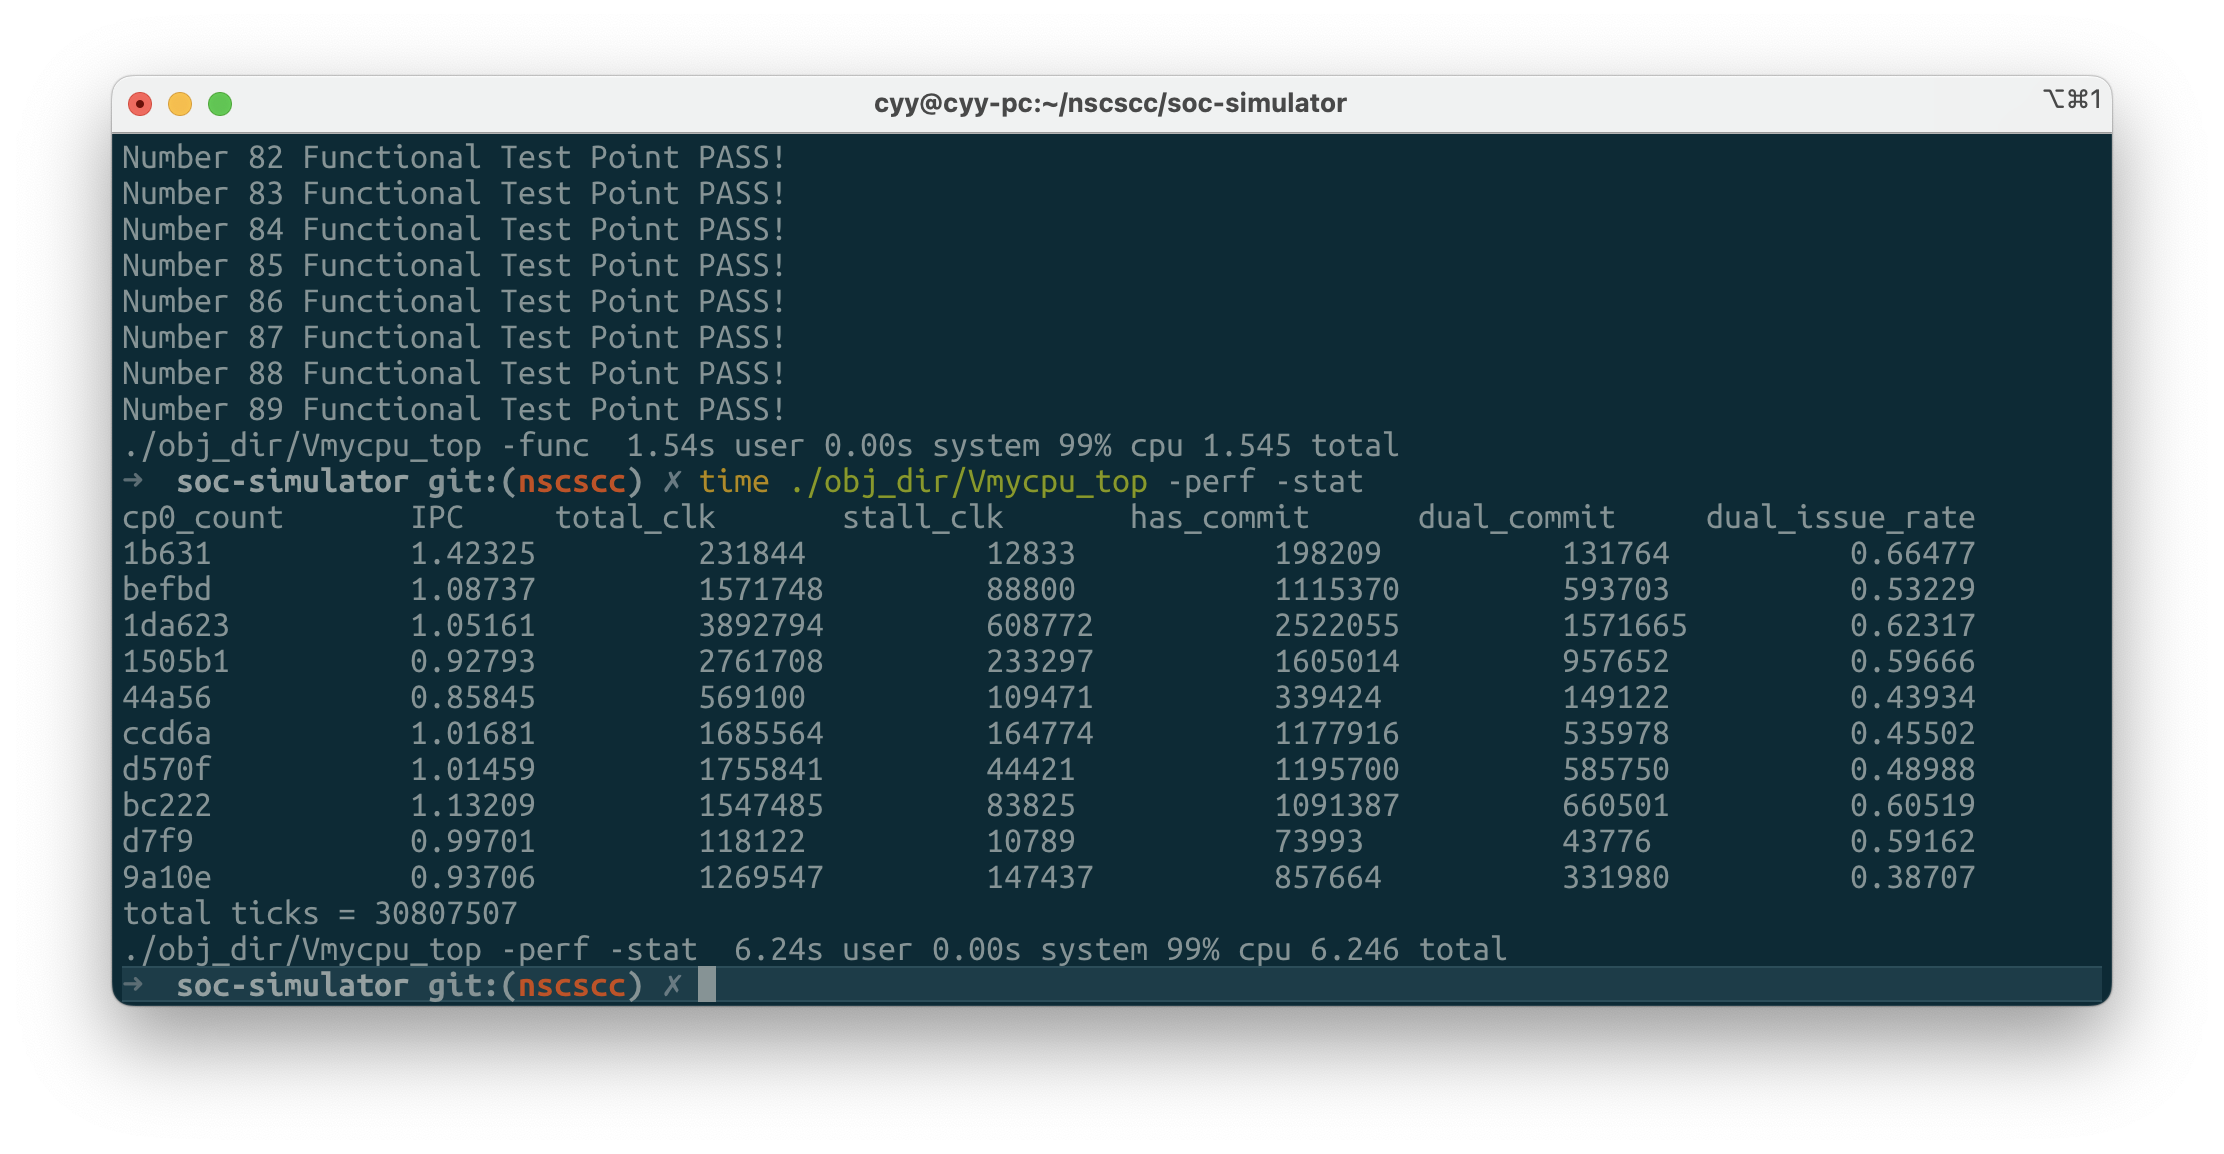
\includegraphics[width=\linewidth]{soc_simulator_func_perf.png}
    \caption{SoC-Simulator运行功能测试与性能测试}
\end{figure}

\begin{figure}[h]
    \centering
    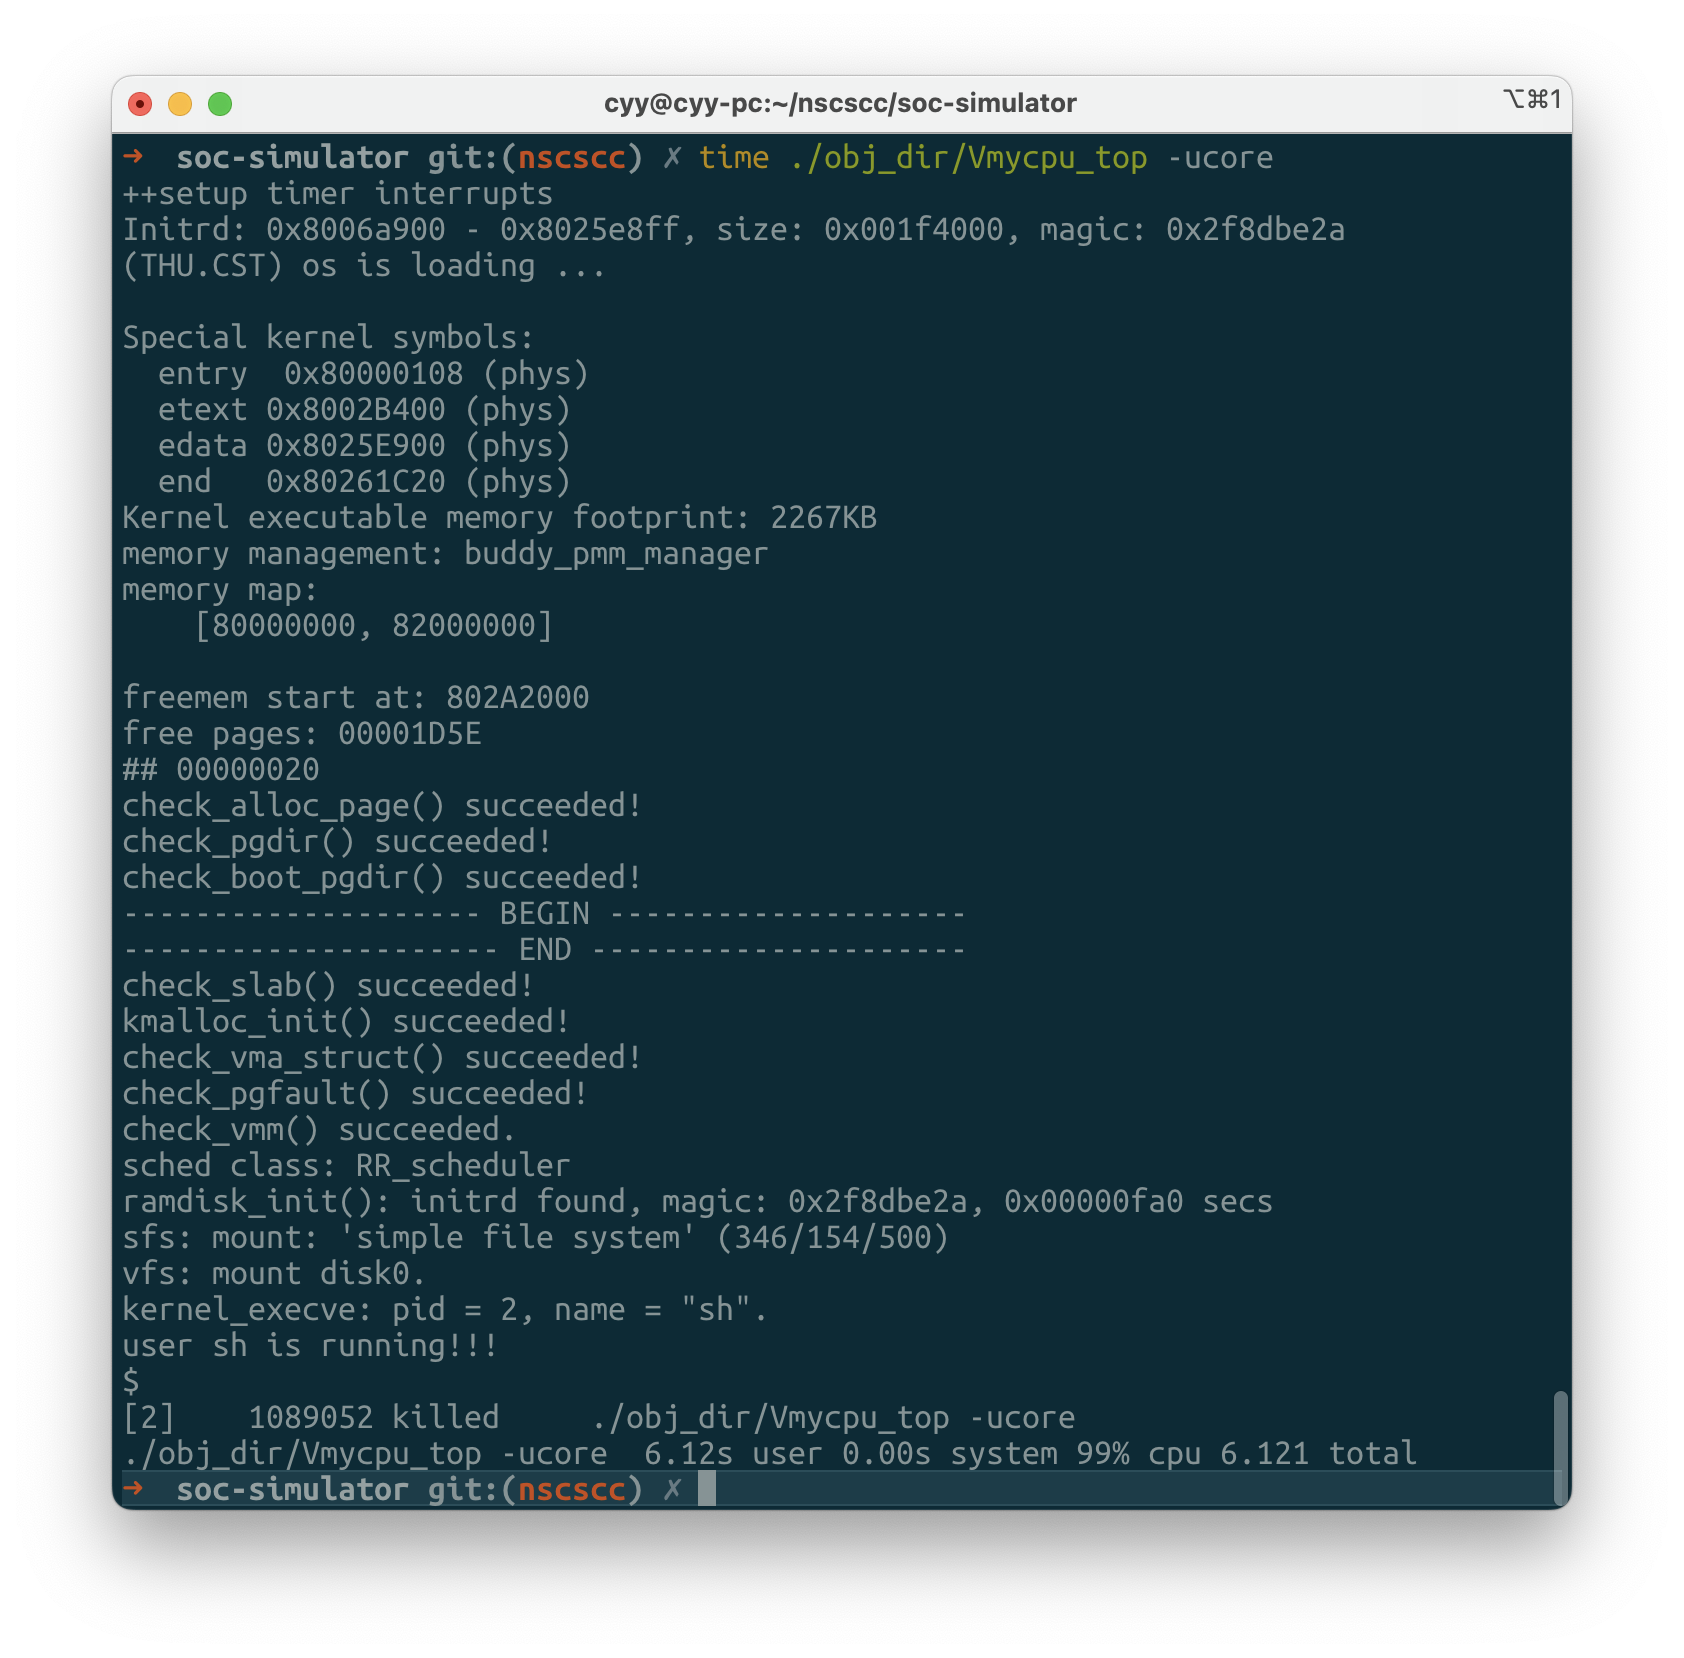
\includegraphics[width=\linewidth]{soc_simulator_ucore.png}
    \caption{SoC-Simulator运行uCore}
\end{figure}

\begin{figure}[h]
    \centering
    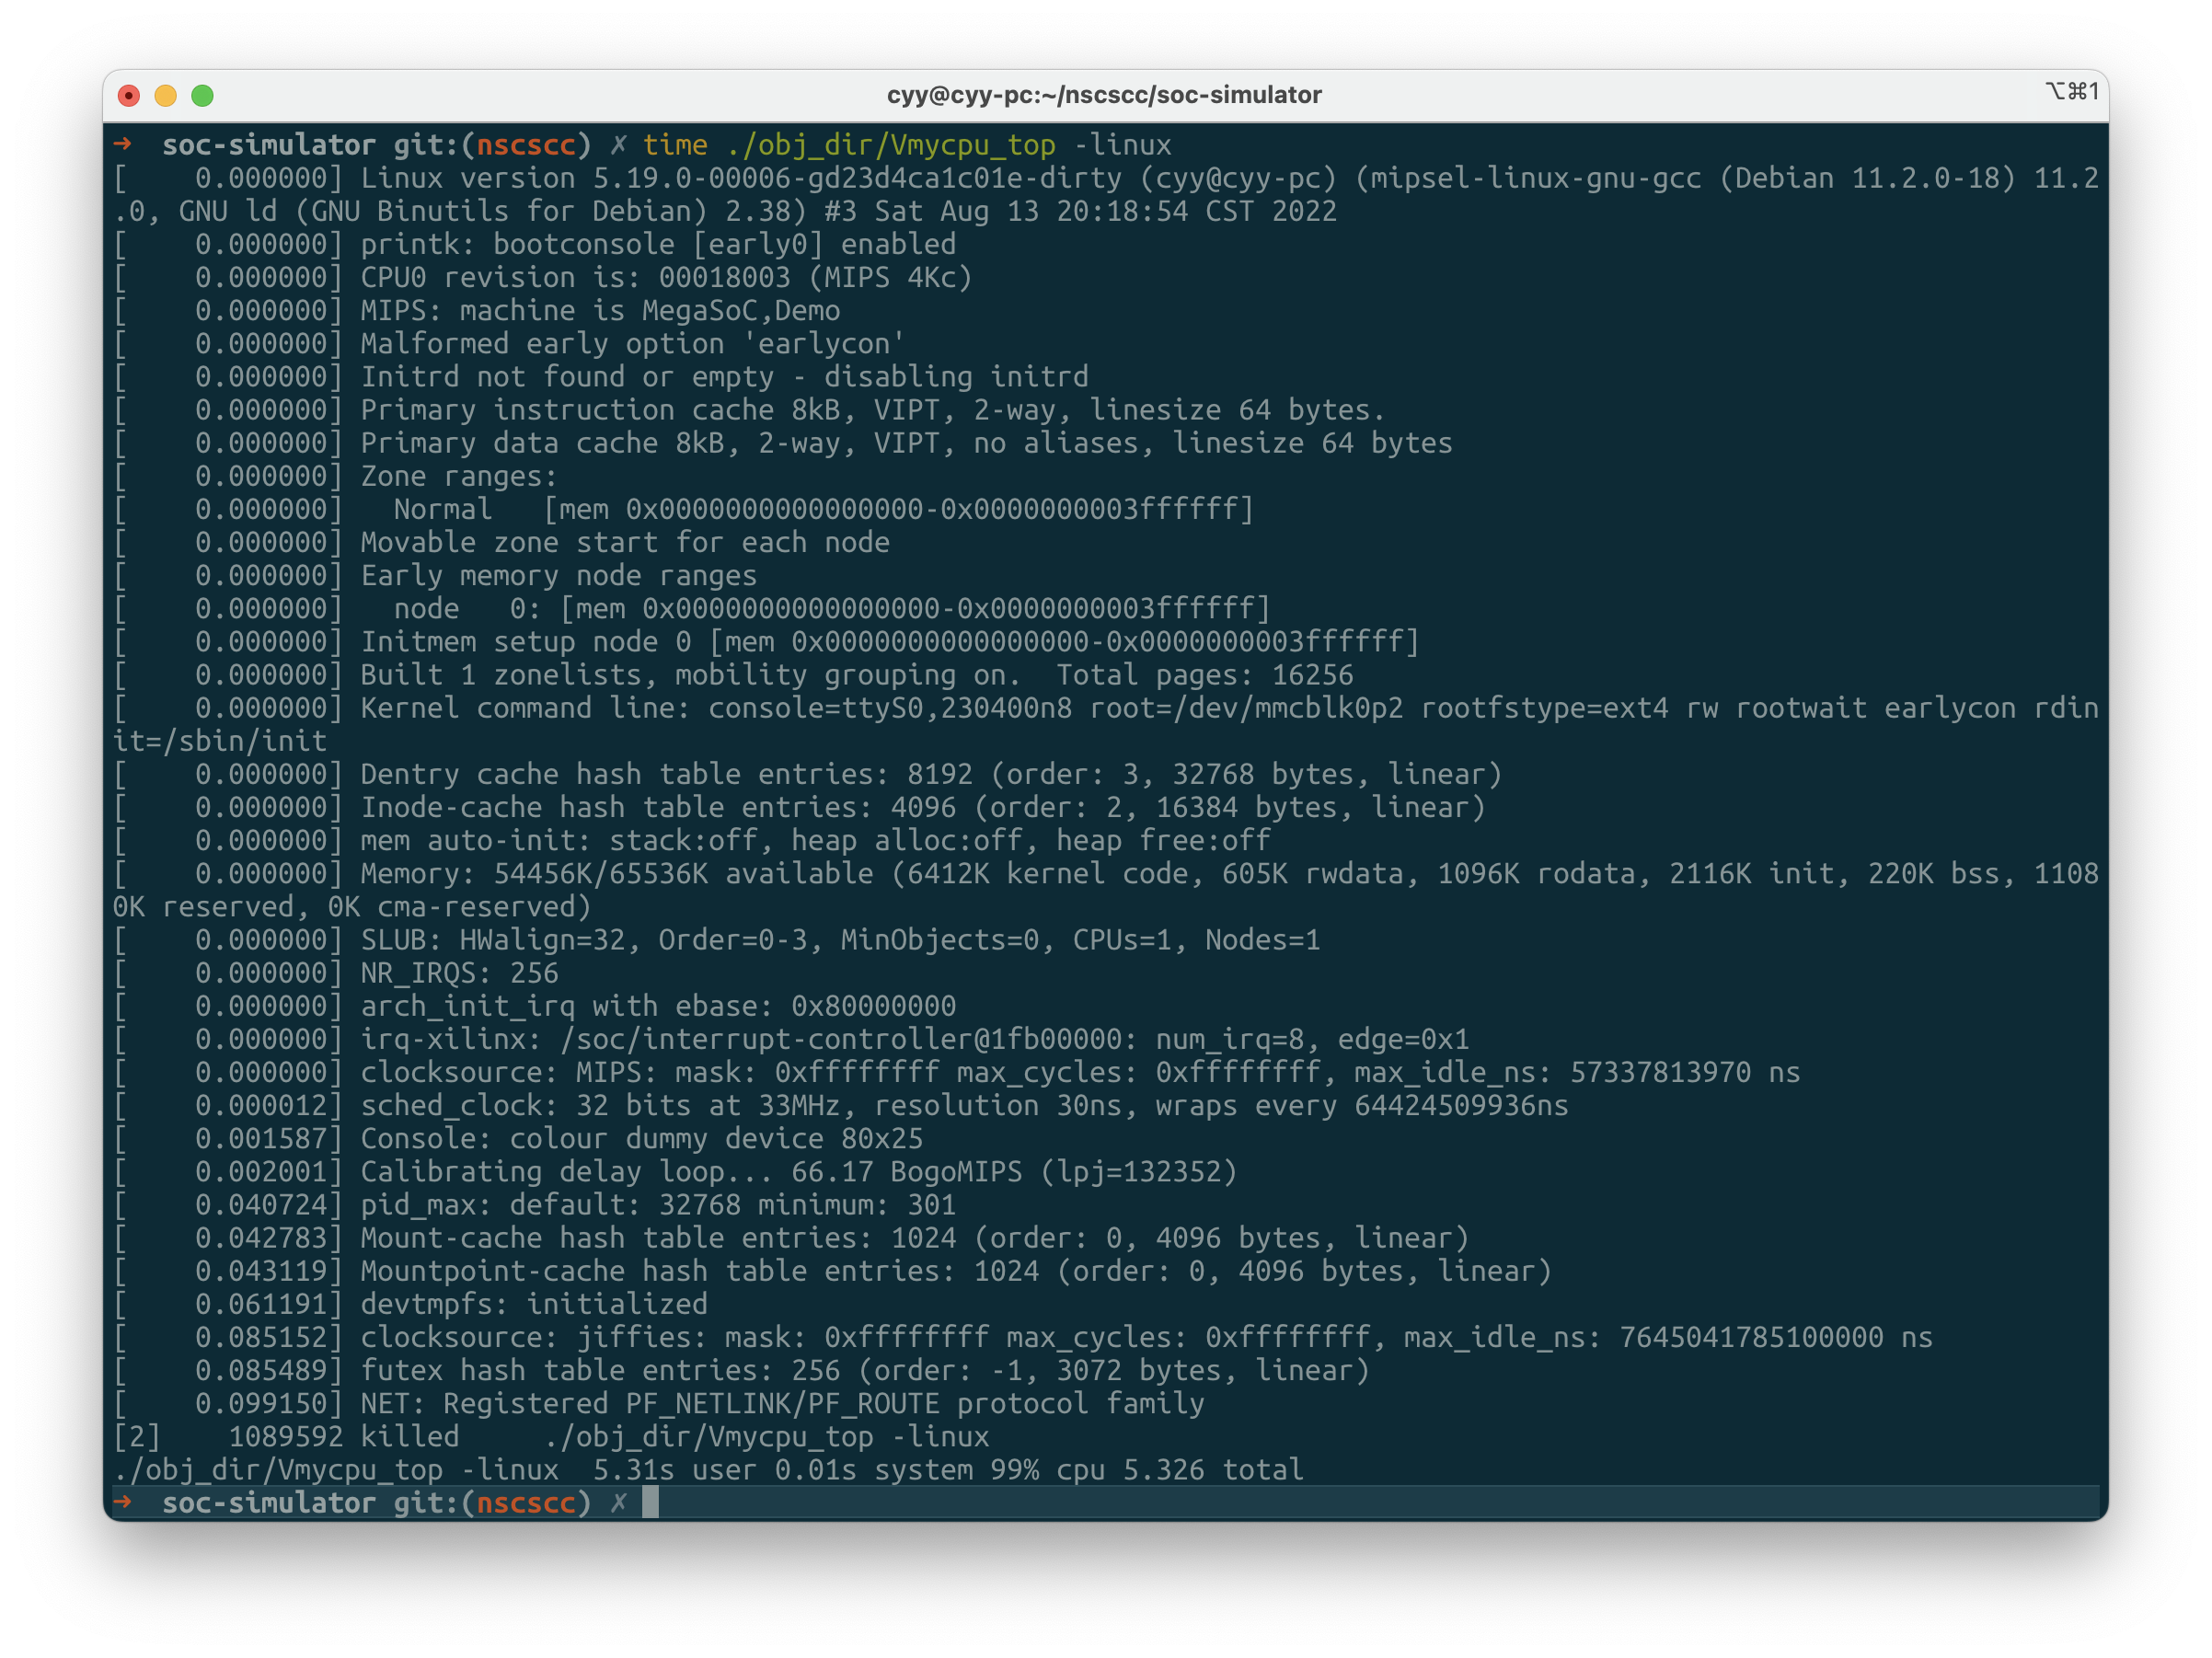
\includegraphics[width=\linewidth]{soc_simulator_linux.png}
    \caption{SoC-Simulator运行Linux}
\end{figure}

\section{CEMU}

CEMU(CQU Emulator)是我们开发的一个CPU模拟器,目前支持了RV64IMA与MIPS Release 1指令集,LoongArch32的支持正在实现中,我们使用它与\cpuname 进行差分测试,

由于CEMU与SoC-Simulator都是我们自行开发的,因而采用了完全相同的外设接口(C++的抽象类),从而CEMU与SoC-Simulator能够运行在完全相同的SoC环境中,并通过处理器RTL输出的CP0 Count、CP0 Cause、CP0 Random、是否中断等信号对CEMU的各寄存器状态进行同步,这帮助我们在\cpuname 调通uCore后仅2天时间就完成了Linux的调试。

在\cpuname 调试过程中,我们也不断完善了CEMU与SoC-Simulator的difftest功能。例如添加了内存写回时AXI传入数据与CEMU内存的对比功能,以及条件输出波形图等功能(避免调试Linux时波形图输出消耗大量存储资源)。并在调试Linux期间为了调试Linux Kernel自身写入的指令(如ebase段的异常处理,这部分不在vmlinux的反汇编中)的执行过程,在差分测试错误时能够将cemu的整个内存转储出来,再通过objdump反汇编即可知道动态写入的指令,便于通过指令序列观察处理器执行可能存在的问题(例如常见的延迟槽出现先前测试未覆盖的指令)。

\begin{figure}[h]
    \centering
    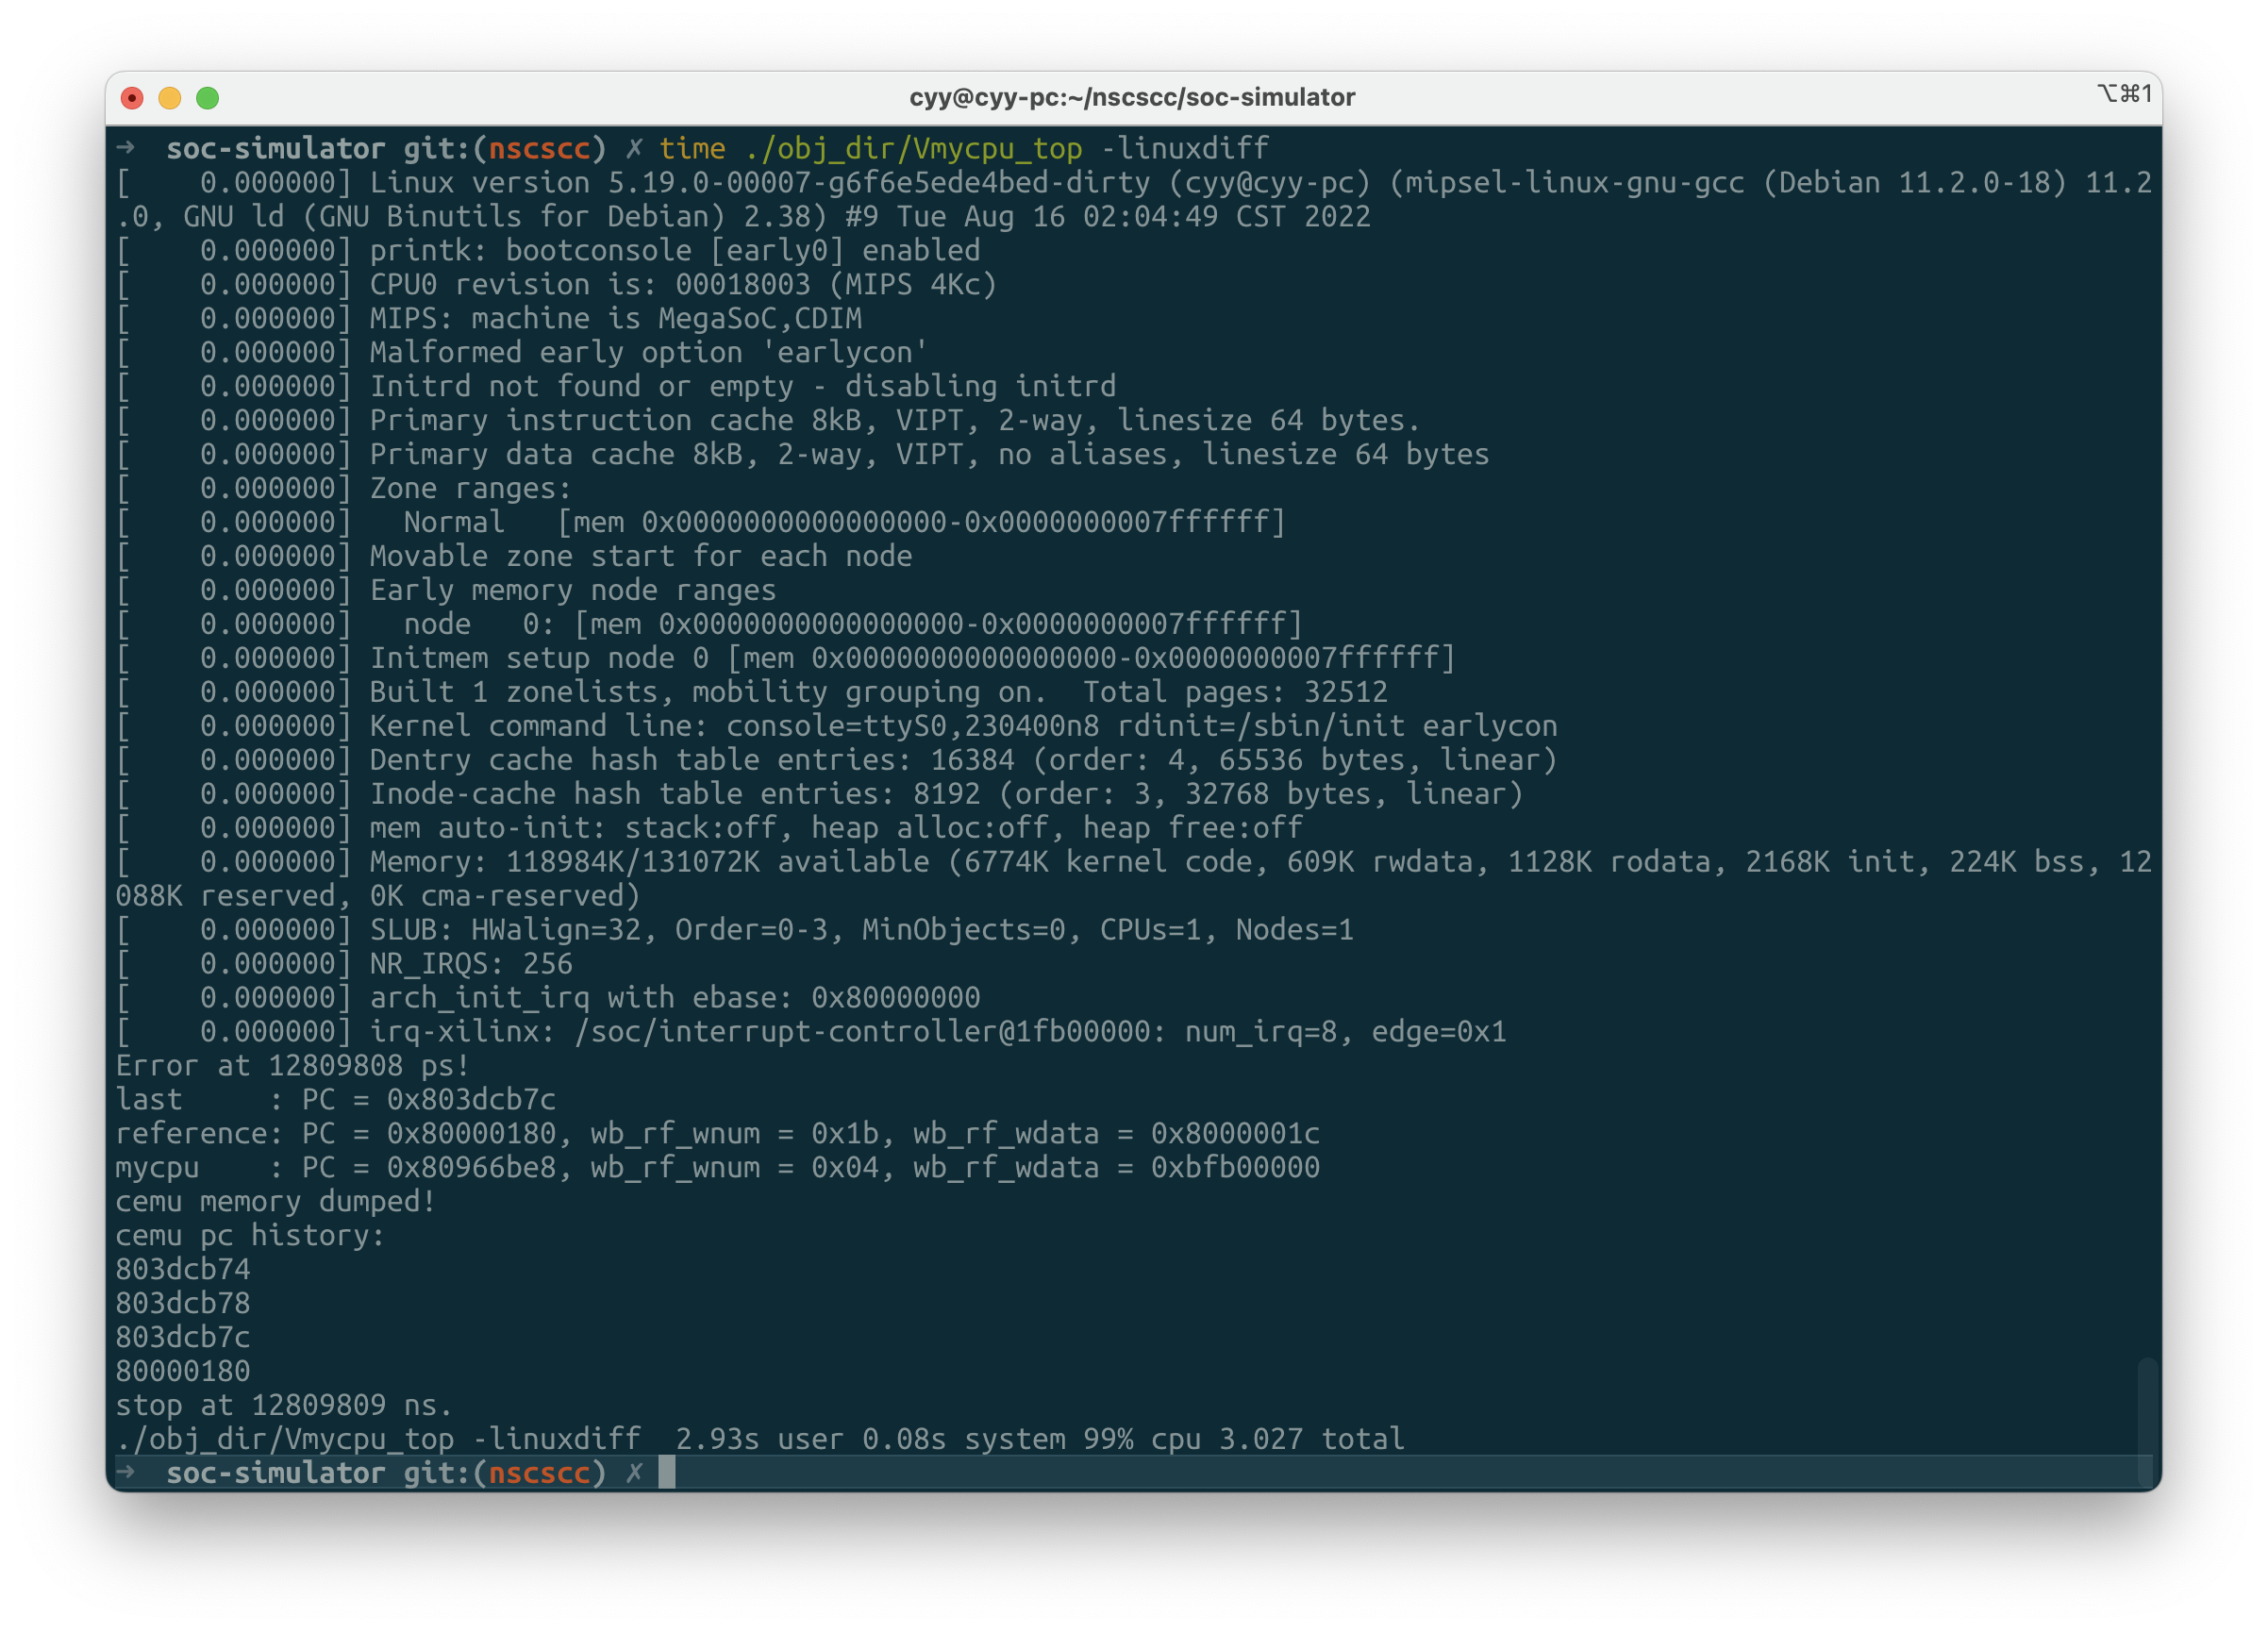
\includegraphics[width=\linewidth]{soc_simulator_linuxdiff.png}
    \caption{SoC-Simulator与CEMU差分测试错误提示}
\end{figure}
\chapter{操作系统支持}

\section{虚拟内存支持}\label{section:TLB}

\cpuname 支持了MIPS规范中基于TLB的虚拟地址转换功能。
由于MIPS指令集架构中,TLB采用全相连的结构,匹配需要大量的电路延迟,为了保证运行操作系统时的频率,我们将TLB拆为两级。

\begin{figure}[h]
    \centering
    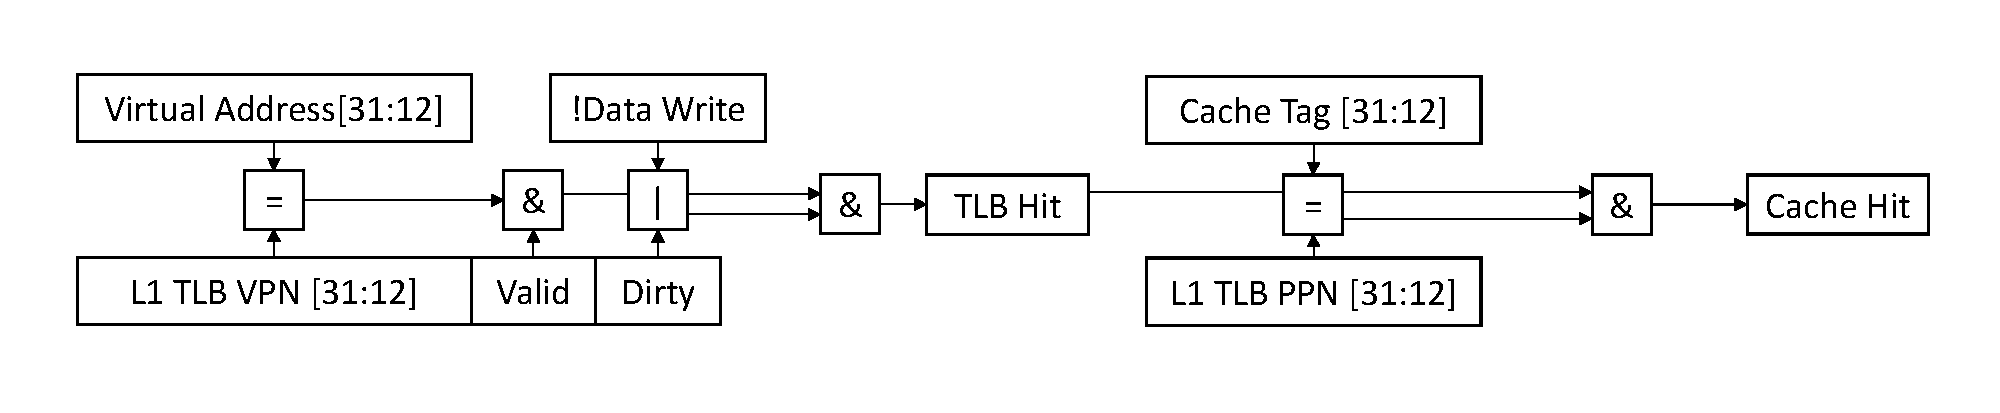
\includegraphics[width=\linewidth]{l1_tlb.pdf}
    \caption{一级TLB的设计}
    \label{img:l1_tlb}
\end{figure}

其中,一级TLB分为一级指令TLB与一级数据TLB,各只有一项,位于指令Cache与数据Cache中。
由于我们的Cache单路恰好为4KB,恰好为我们处理器支持的最小页面大小,因此采用伪VIPT(Virtually Indexed Physically Tagged)方式,比较方式如图\ref{img:l1_tlb}所示。

在我们的设计中,一级TLB与Cache状态机深度整合,且在一级TLB命中的情况下不会带来额外的流水线停顿,由此兼顾了IPC与频率。

二级TLB采用全相连结构,有8项,位于CP0中,提供了3个可同时访问的查找接口分别用于TLBP指令、一级指令TLB、一级数据TLB。
当一级TLB缺失时,会向CP0中的L2 TLB发出缺失的VPN2地址(虚拟地址的[31:27]部分)进行TLB查找,并在下一周期得到对应的TLB表项以及是否命中成功。
当出现L2 TLB查找失败、TLB无效、写只读页等情况时,则根据当前状态发出对应的异常,跳转到异常处理地址交给系统内核完成TLB的回填操作。

由于我们TLB做了两级,需要解决L1 TLB与L2 TLB间的一致性问题,这里需要考虑两种情况,一种是ASID切换,另一种是TLB写入。
我们采用的设计是在L1 TLB中添加一个清空TLB的信号,并在执行MTC0、TLBWI、TLBWR三条指令时都拉高清空信号,以解决虚拟地址重名问题。

\section{Cache指令支持}

由于操作系统中存在写入指令后执行,与DMA前后写回或失效Cache的操作,这需要Cache指令的支持。这一部分已在Cache章节有所介绍。
且经过我们测试发现Linux不会使用Index Store Tag这样特殊的Cache指令,因此这样简单的实现就满足了运行Linux的要求。

\section{U-Boot}

我们继承了前辈NSCSCC 2019 清华大学 编程是一件很危险的事情 与 NSCSCC 2021 北京航空航天大学一队的工作,为我们的CPU移植的U-Boot。
主要工作包括编写设备树、修改配置文件、修改串口时钟频率。最终我们成功运行起了U-Boot并能够通过tftp载入uCore与Linux操作系统。

\begin{figure}[h]
    \centering
    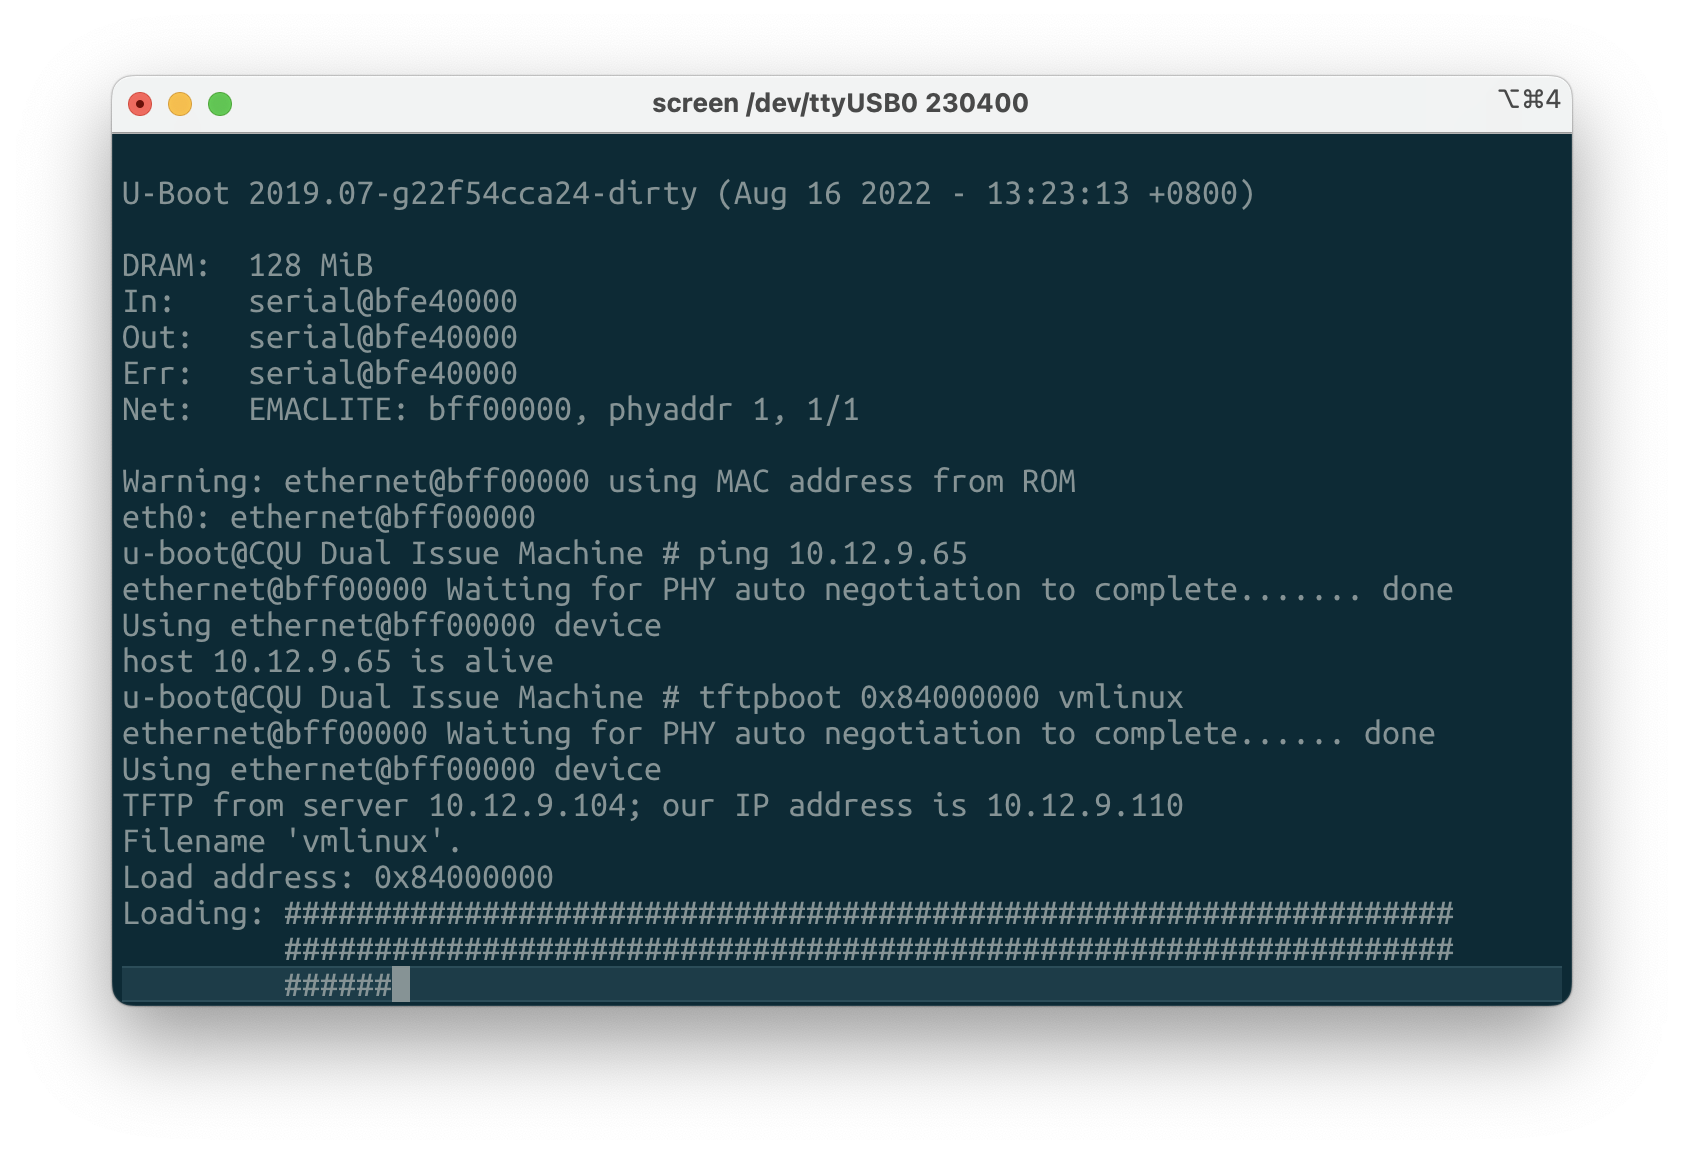
\includegraphics[width=\linewidth]{u-boot.png}
    \caption{U-Boot启动截图}
\end{figure}

\newpage

\section{uCore}

我们的处理器能够运行清华大学的教学操作系统uCore,并进入用户Shell执行程序。

\begin{figure}[htpb]
    \centering
    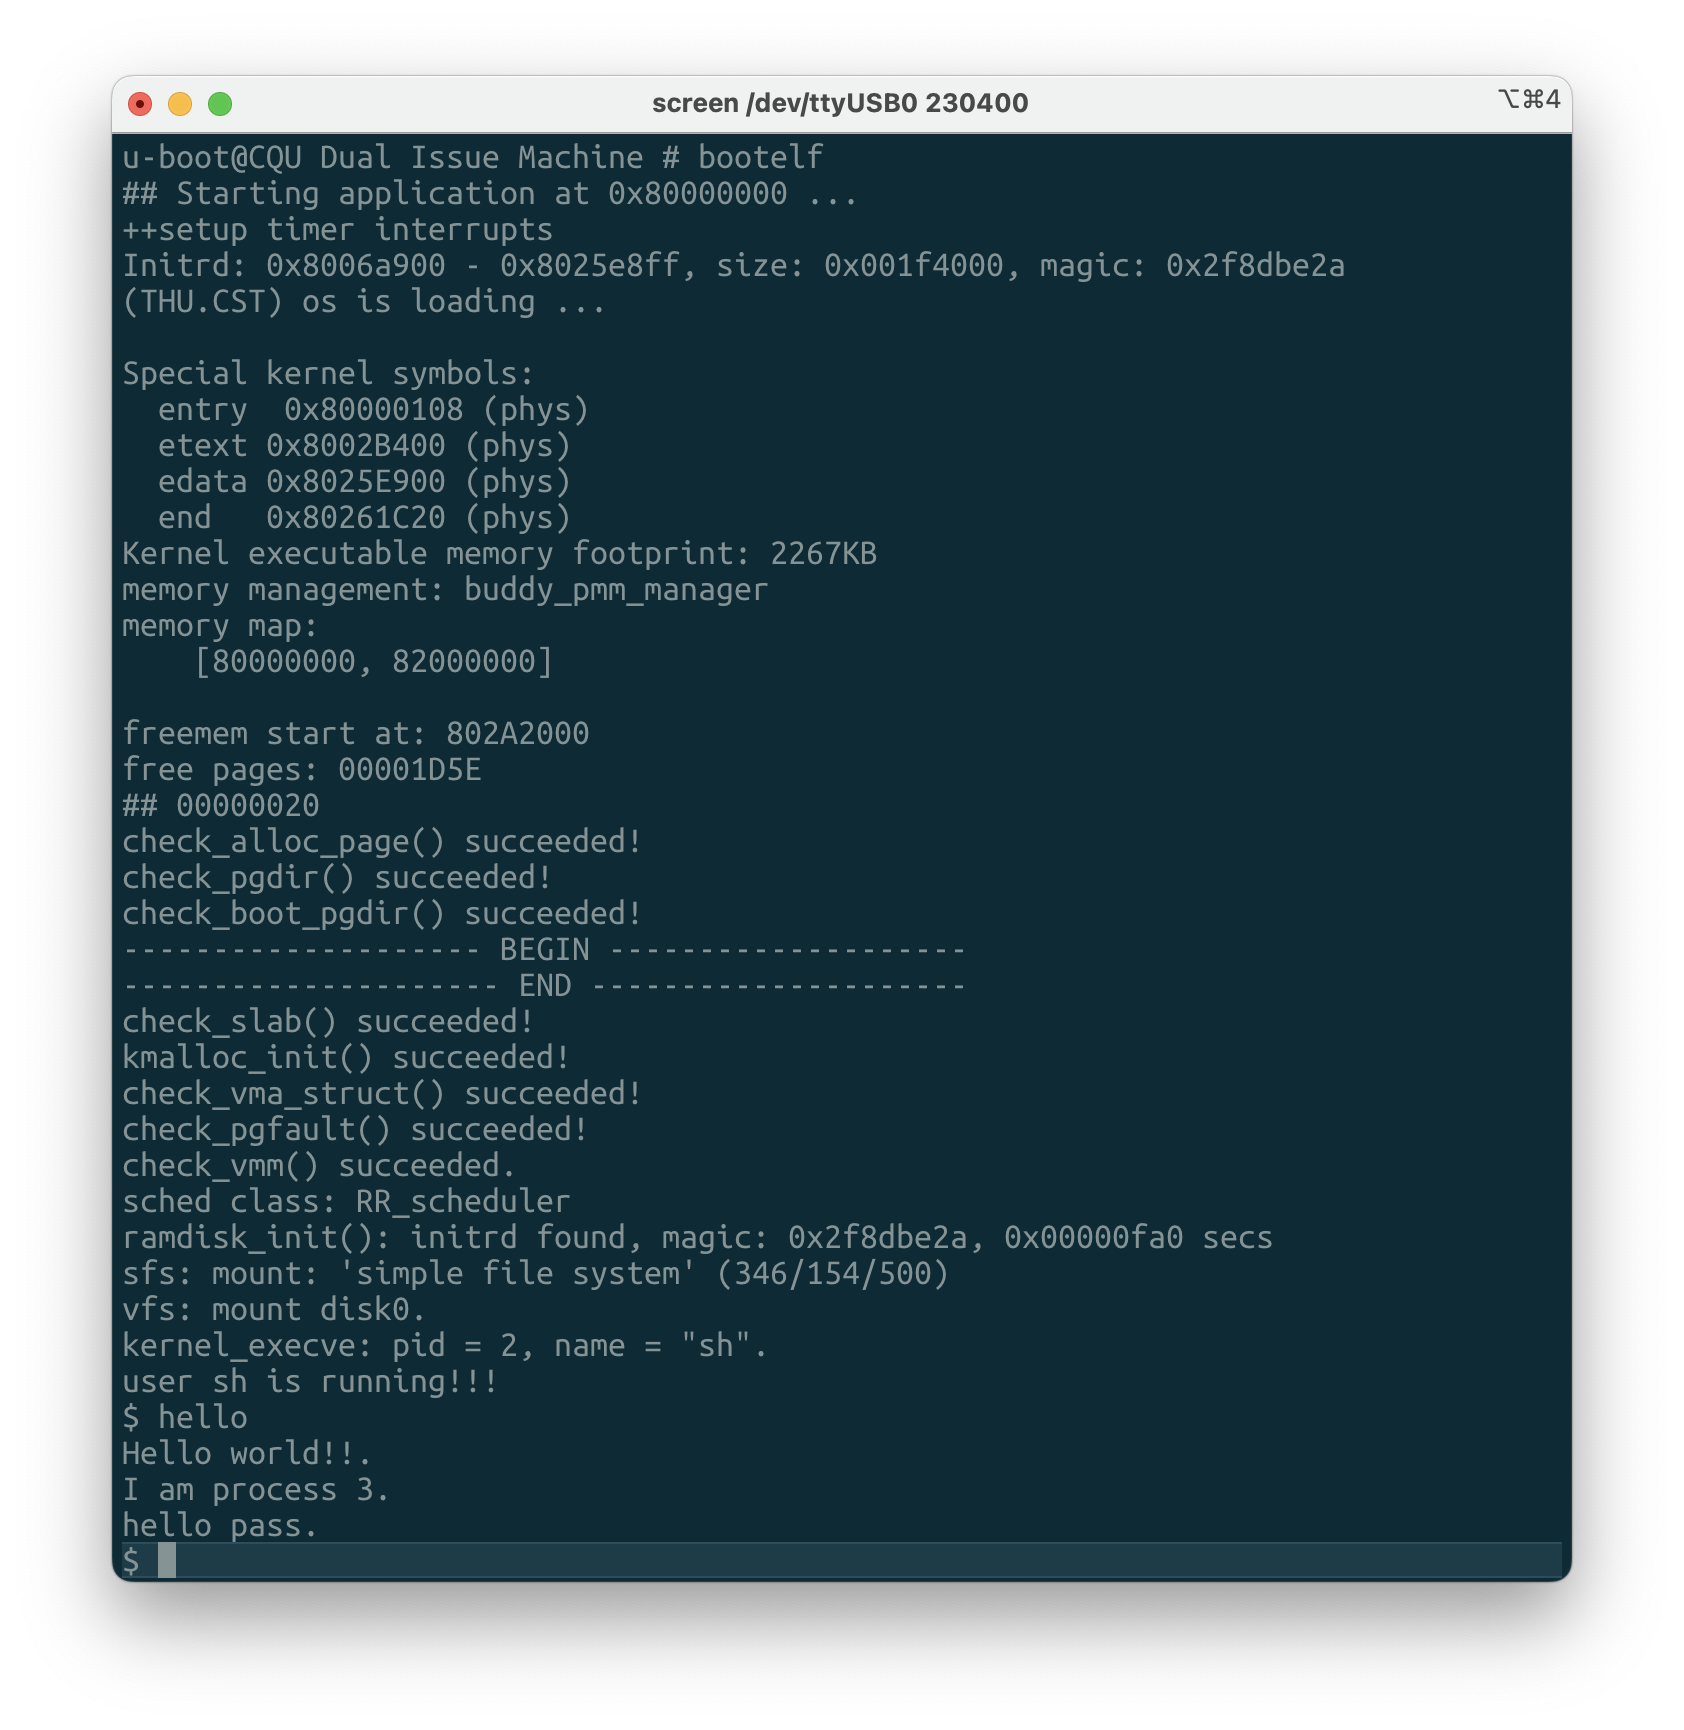
\includegraphics[width=\linewidth]{ucore.png}
    \caption{uCore运行截图}
    \label{img:ucore}
\end{figure}

\newpage

\section{Linux}

我们的处理器能够在编译器关闭Branch-Likely指令的情况下运行Linux v5.19,并自己编译了MIPS Release 1关闭浮点支持的Busybox,在Busybox中能够正常使用Shell。

在仿真SoC-Simulator与上板MegaSoC SoC上均测试成功,且能够使用SoC上的AXI Ethernet Lite IP核连接网络,能够使用wget访问www.nscscc.com网站并提取部分文字。

\begin{figure}[h]
    \centering
    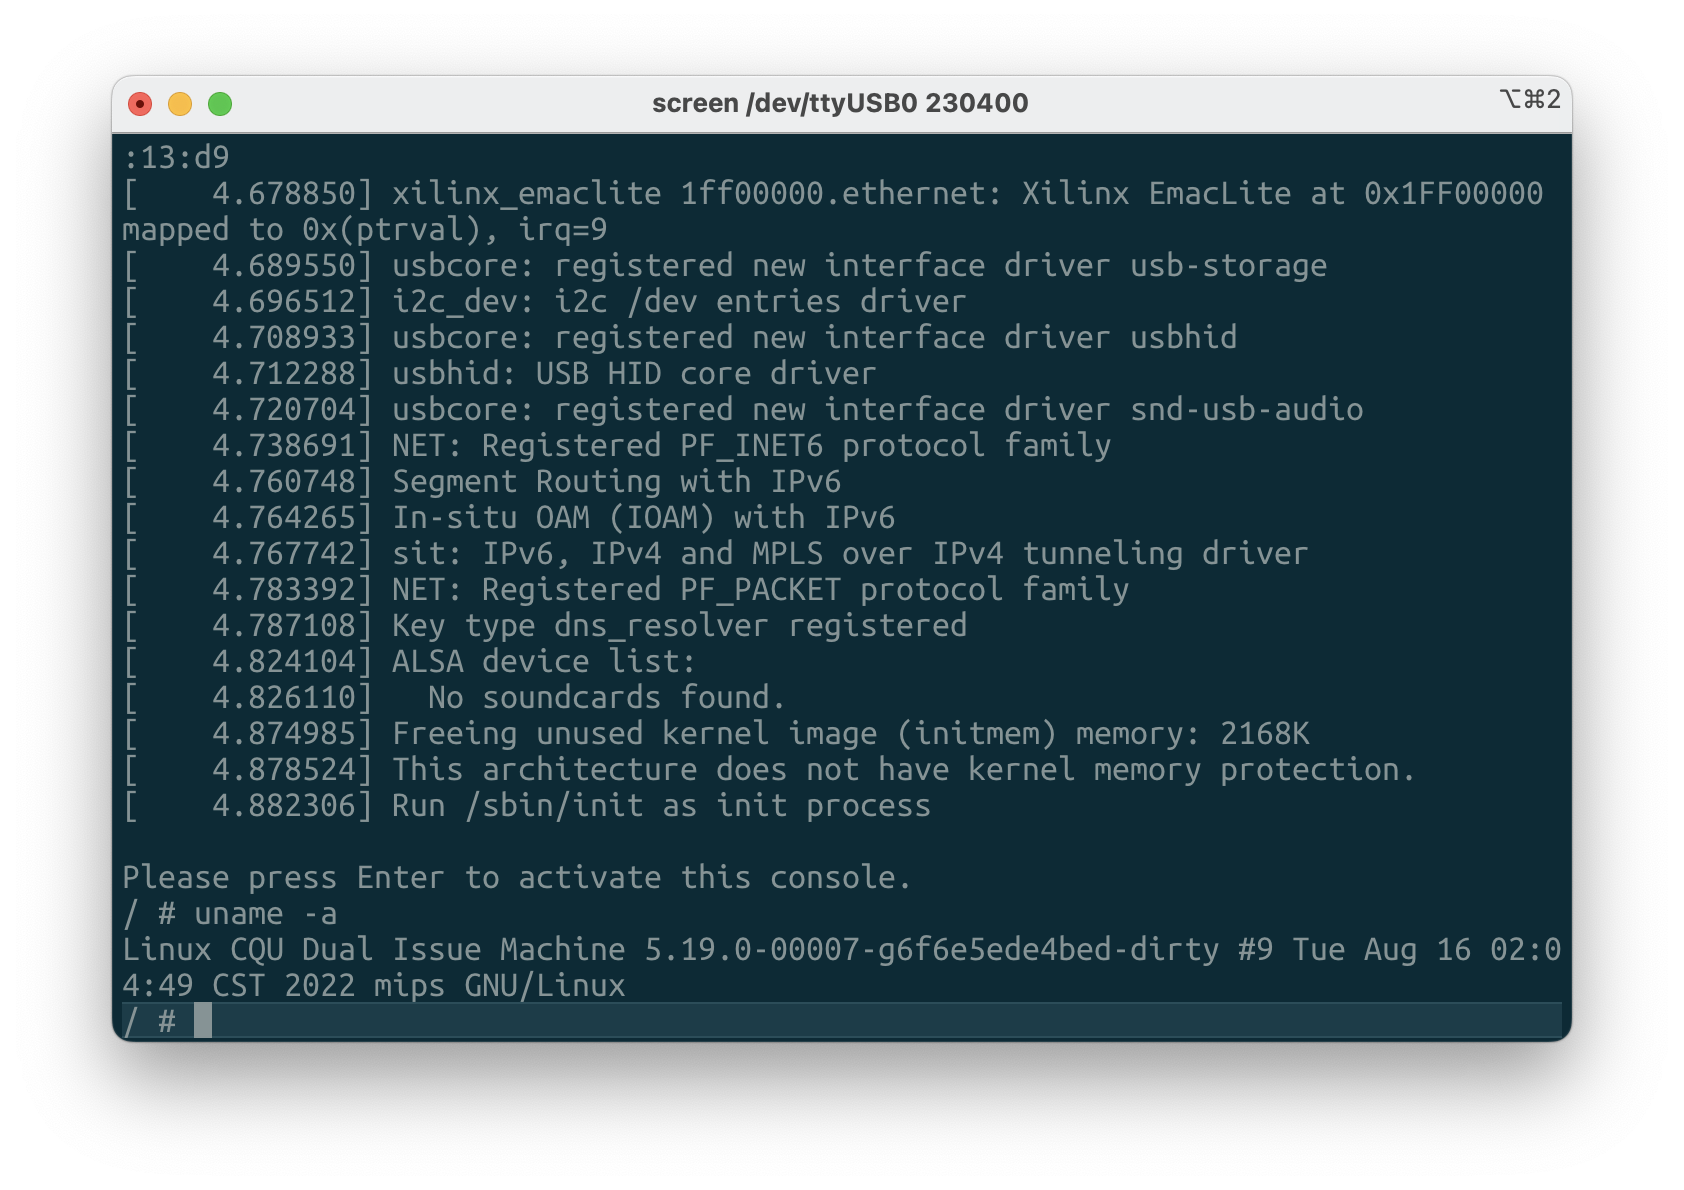
\includegraphics[width=\linewidth]{linux_boot.png}
    \caption{Linux启动截图}
    \label{img:linux_boot}
\end{figure}

\begin{figure}[h]
    \centering
    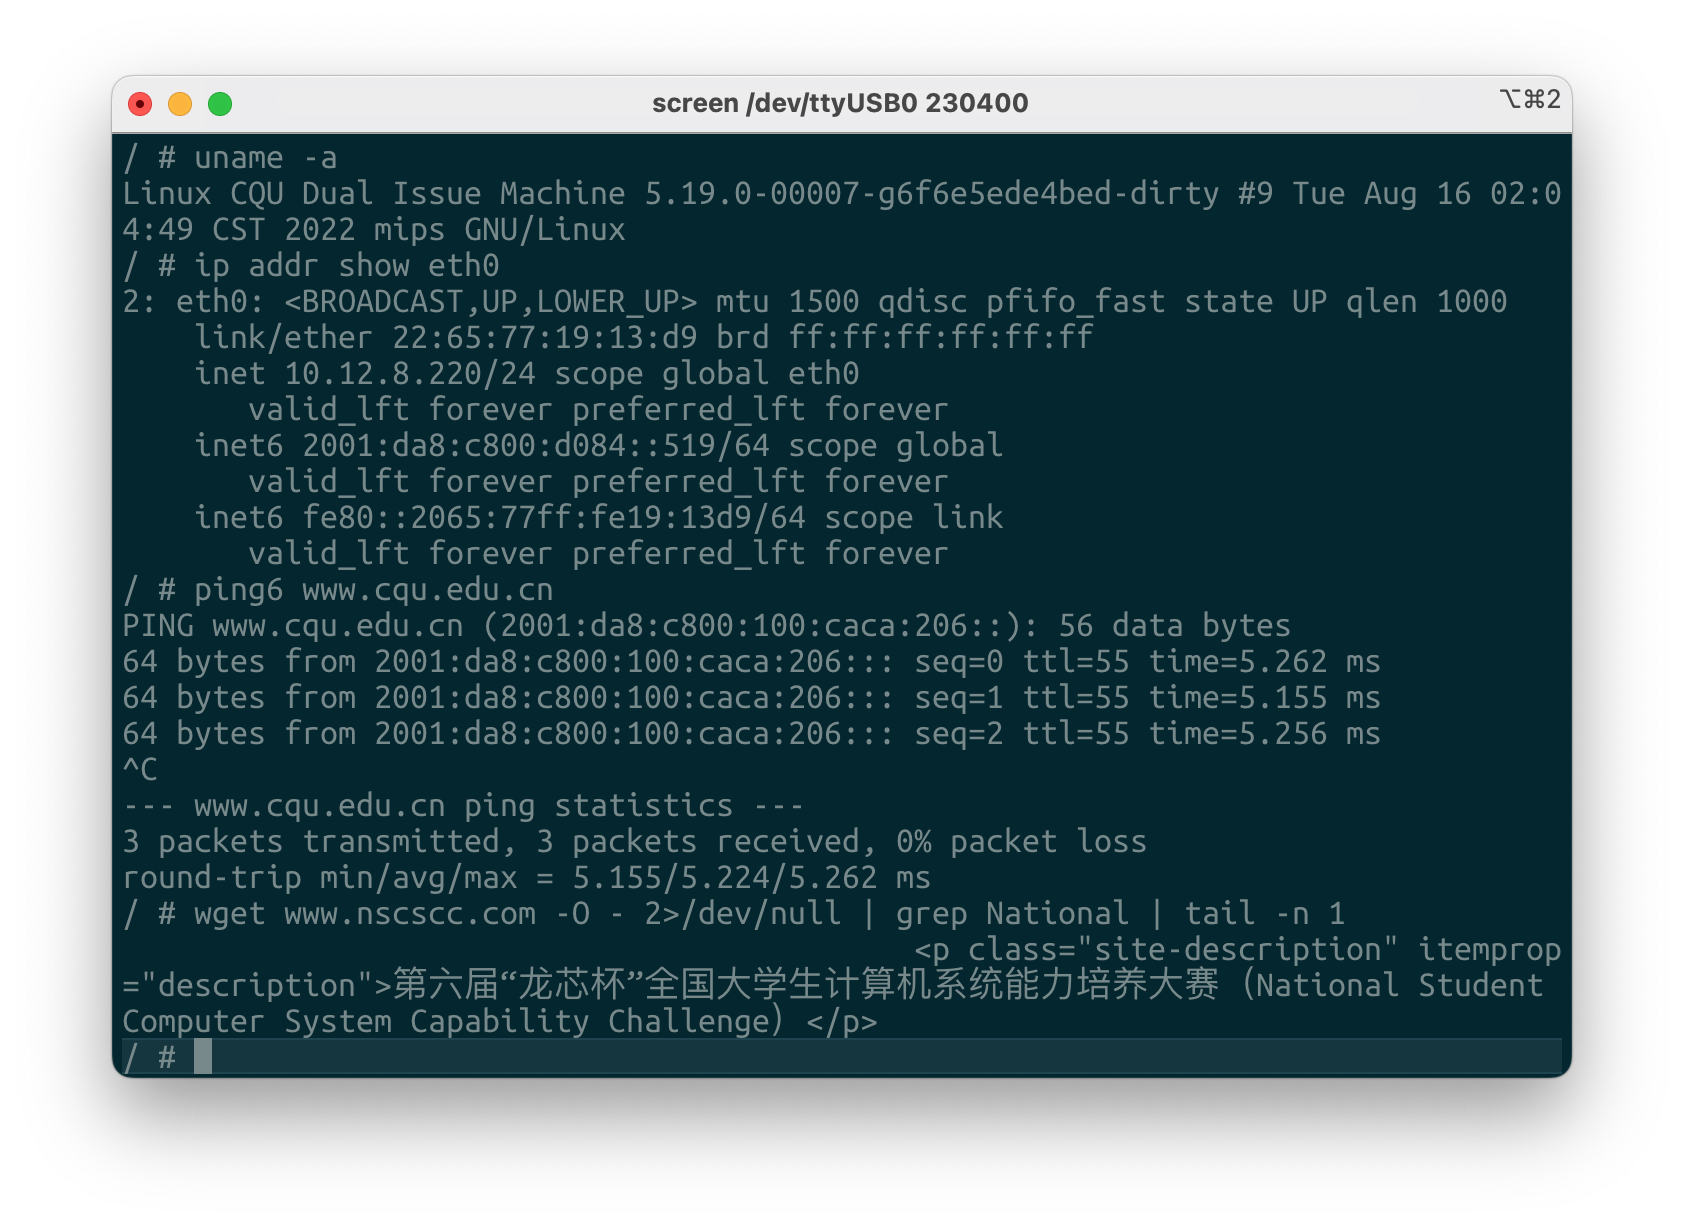
\includegraphics[width=\linewidth]{linux_nic_test.png}
    \caption{Linux上网截图}
    \label{img:linux_nic_test}
\end{figure}
\chapter{附录}

\section{系统软件移植仓库}

\begin{table}[!htbp]
    \centering
    \caption{系统软件移植仓库}
    
    \begin{tabular}{cll}
    \toprule
    \multicolumn{1}{c}{\textbf{软件名称}} & \multicolumn{1}{c}{\textbf{代码仓库}} \\ 
    \midrule
    U-Boot                             & \url{https://github.com/cyyself/u-boot/commits/cdim\_soc} \\
    uCore                              & \url{https://github.com/cyyself/ucore-thumips/tree/cdim\_soc} \\
    Linux                              & \url{https://github.com/cyyself/linux/tree/cdim\_soc} \\
    \bottomrule
    \end{tabular}
\end{table}

\section{差分测试工具链}

\begin{table}[!htbp]
    \centering
    \caption{差分测试工具链}
    
    \begin{tabular}{cll}
    \toprule
    \multicolumn{1}{c}{\textbf{工具名称}} & \multicolumn{1}{c}{\textbf{代码仓库}} \\ 
    \midrule
    SoC-Simulator                      & \url{https://github.com/cyyself/soc-simulator/tree/nscscc} \\
    CEMU                               & \url{https://github.com/cyyself/cemu/tree/mips32-nscscc} \\
    \bottomrule
    \end{tabular}
\end{table}
% 做了就可以说



\newpage
\renewcommand{\bibname}{参考资料}
\begin{thebibliography}{99}
	\bibitem[1]{MIPS} MIPS® Architecture For Programmers I, II, III. Imagination Technologies LTD.  
  \bibitem[2]{HSport} 计算机组成与设计: 硬件/软件接口. David A.Patterson
  \bibitem[3]{Siris} Sirius 设计文档. 于海鑫,尹思维
  \bibitem[4]{SelfCPU} 自己动手写 CPU. 雷思磊
  \bibitem[5]{MegaSoC} MegaSoC \url{https://github.com/MegaSoC}
\end{thebibliography}



\end{document}